
\documentclass{article} % For LaTeX2e
\usepackage{iclr2027_conference,times}

% Optional math commands from https://github.com/goodfeli/dlbook_notation.
%%%%% NEW MATH DEFINITIONS %%%%%

\usepackage{amsmath,amsfonts,bm}

% Mark sections of captions for referring to divisions of figures
\newcommand{\figleft}{{\em (Left)}}
\newcommand{\figcenter}{{\em (Center)}}
\newcommand{\figright}{{\em (Right)}}
\newcommand{\figtop}{{\em (Top)}}
\newcommand{\figbottom}{{\em (Bottom)}}
\newcommand{\captiona}{{\em (a)}}
\newcommand{\captionb}{{\em (b)}}
\newcommand{\captionc}{{\em (c)}}
\newcommand{\captiond}{{\em (d)}}

% Highlight a newly defined term
\newcommand{\newterm}[1]{{\bf #1}}


% Figure reference, lower-case.
\def\figref#1{figure~\ref{#1}}
% Figure reference, capital. For start of sentence
\def\Figref#1{Figure~\ref{#1}}
\def\twofigref#1#2{figures \ref{#1} and \ref{#2}}
\def\quadfigref#1#2#3#4{figures \ref{#1}, \ref{#2}, \ref{#3} and \ref{#4}}
% Section reference, lower-case.
\def\secref#1{section~\ref{#1}}
% Section reference, capital.
\def\Secref#1{Section~\ref{#1}}
% Reference to two sections.
\def\twosecrefs#1#2{sections \ref{#1} and \ref{#2}}
% Reference to three sections.
\def\secrefs#1#2#3{sections \ref{#1}, \ref{#2} and \ref{#3}}
% Reference to an equation, lower-case.
\def\eqref#1{equation~\ref{#1}}
% Reference to an equation, upper case
\def\Eqref#1{Equation~\ref{#1}}
% A raw reference to an equation---avoid using if possible
\def\plaineqref#1{\ref{#1}}
% Reference to a chapter, lower-case.
\def\chapref#1{chapter~\ref{#1}}
% Reference to an equation, upper case.
\def\Chapref#1{Chapter~\ref{#1}}
% Reference to a range of chapters
\def\rangechapref#1#2{chapters\ref{#1}--\ref{#2}}
% Reference to an algorithm, lower-case.
\def\algref#1{algorithm~\ref{#1}}
% Reference to an algorithm, upper case.
\def\Algref#1{Algorithm~\ref{#1}}
\def\twoalgref#1#2{algorithms \ref{#1} and \ref{#2}}
\def\Twoalgref#1#2{Algorithms \ref{#1} and \ref{#2}}
% Reference to a part, lower case
\def\partref#1{part~\ref{#1}}
% Reference to a part, upper case
\def\Partref#1{Part~\ref{#1}}
\def\twopartref#1#2{parts \ref{#1} and \ref{#2}}

\def\ceil#1{\lceil #1 \rceil}
\def\floor#1{\lfloor #1 \rfloor}
\def\1{\bm{1}}
\newcommand{\train}{\mathcal{D}}
\newcommand{\valid}{\mathcal{D_{\mathrm{valid}}}}
\newcommand{\test}{\mathcal{D_{\mathrm{test}}}}

\def\eps{{\epsilon}}


% Random variables
\def\reta{{\textnormal{$\eta$}}}
\def\ra{{\textnormal{a}}}
\def\rb{{\textnormal{b}}}
\def\rc{{\textnormal{c}}}
\def\rd{{\textnormal{d}}}
\def\re{{\textnormal{e}}}
\def\rf{{\textnormal{f}}}
\def\rg{{\textnormal{g}}}
\def\rh{{\textnormal{h}}}
\def\ri{{\textnormal{i}}}
\def\rj{{\textnormal{j}}}
\def\rk{{\textnormal{k}}}
\def\rl{{\textnormal{l}}}
% rm is already a command, just don't name any random variables m
\def\rn{{\textnormal{n}}}
\def\ro{{\textnormal{o}}}
\def\rp{{\textnormal{p}}}
\def\rq{{\textnormal{q}}}
\def\rr{{\textnormal{r}}}
\def\rs{{\textnormal{s}}}
\def\rt{{\textnormal{t}}}
\def\ru{{\textnormal{u}}}
\def\rv{{\textnormal{v}}}
\def\rw{{\textnormal{w}}}
\def\rx{{\textnormal{x}}}
\def\ry{{\textnormal{y}}}
\def\rz{{\textnormal{z}}}

% Random vectors
\def\rvepsilon{{\mathbf{\epsilon}}}
\def\rvtheta{{\mathbf{\theta}}}
\def\rva{{\mathbf{a}}}
\def\rvb{{\mathbf{b}}}
\def\rvc{{\mathbf{c}}}
\def\rvd{{\mathbf{d}}}
\def\rve{{\mathbf{e}}}
\def\rvf{{\mathbf{f}}}
\def\rvg{{\mathbf{g}}}
\def\rvh{{\mathbf{h}}}
\def\rvu{{\mathbf{i}}}
\def\rvj{{\mathbf{j}}}
\def\rvk{{\mathbf{k}}}
\def\rvl{{\mathbf{l}}}
\def\rvm{{\mathbf{m}}}
\def\rvn{{\mathbf{n}}}
\def\rvo{{\mathbf{o}}}
\def\rvp{{\mathbf{p}}}
\def\rvq{{\mathbf{q}}}
\def\rvr{{\mathbf{r}}}
\def\rvs{{\mathbf{s}}}
\def\rvt{{\mathbf{t}}}
\def\rvu{{\mathbf{u}}}
\def\rvv{{\mathbf{v}}}
\def\rvw{{\mathbf{w}}}
\def\rvx{{\mathbf{x}}}
\def\rvy{{\mathbf{y}}}
\def\rvz{{\mathbf{z}}}

% Elements of random vectors
\def\erva{{\textnormal{a}}}
\def\ervb{{\textnormal{b}}}
\def\ervc{{\textnormal{c}}}
\def\ervd{{\textnormal{d}}}
\def\erve{{\textnormal{e}}}
\def\ervf{{\textnormal{f}}}
\def\ervg{{\textnormal{g}}}
\def\ervh{{\textnormal{h}}}
\def\ervi{{\textnormal{i}}}
\def\ervj{{\textnormal{j}}}
\def\ervk{{\textnormal{k}}}
\def\ervl{{\textnormal{l}}}
\def\ervm{{\textnormal{m}}}
\def\ervn{{\textnormal{n}}}
\def\ervo{{\textnormal{o}}}
\def\ervp{{\textnormal{p}}}
\def\ervq{{\textnormal{q}}}
\def\ervr{{\textnormal{r}}}
\def\ervs{{\textnormal{s}}}
\def\ervt{{\textnormal{t}}}
\def\ervu{{\textnormal{u}}}
\def\ervv{{\textnormal{v}}}
\def\ervw{{\textnormal{w}}}
\def\ervx{{\textnormal{x}}}
\def\ervy{{\textnormal{y}}}
\def\ervz{{\textnormal{z}}}

% Random matrices
\def\rmA{{\mathbf{A}}}
\def\rmB{{\mathbf{B}}}
\def\rmC{{\mathbf{C}}}
\def\rmD{{\mathbf{D}}}
\def\rmE{{\mathbf{E}}}
\def\rmF{{\mathbf{F}}}
\def\rmG{{\mathbf{G}}}
\def\rmH{{\mathbf{H}}}
\def\rmI{{\mathbf{I}}}
\def\rmJ{{\mathbf{J}}}
\def\rmK{{\mathbf{K}}}
\def\rmL{{\mathbf{L}}}
\def\rmM{{\mathbf{M}}}
\def\rmN{{\mathbf{N}}}
\def\rmO{{\mathbf{O}}}
\def\rmP{{\mathbf{P}}}
\def\rmQ{{\mathbf{Q}}}
\def\rmR{{\mathbf{R}}}
\def\rmS{{\mathbf{S}}}
\def\rmT{{\mathbf{T}}}
\def\rmU{{\mathbf{U}}}
\def\rmV{{\mathbf{V}}}
\def\rmW{{\mathbf{W}}}
\def\rmX{{\mathbf{X}}}
\def\rmY{{\mathbf{Y}}}
\def\rmZ{{\mathbf{Z}}}

% Elements of random matrices
\def\ermA{{\textnormal{A}}}
\def\ermB{{\textnormal{B}}}
\def\ermC{{\textnormal{C}}}
\def\ermD{{\textnormal{D}}}
\def\ermE{{\textnormal{E}}}
\def\ermF{{\textnormal{F}}}
\def\ermG{{\textnormal{G}}}
\def\ermH{{\textnormal{H}}}
\def\ermI{{\textnormal{I}}}
\def\ermJ{{\textnormal{J}}}
\def\ermK{{\textnormal{K}}}
\def\ermL{{\textnormal{L}}}
\def\ermM{{\textnormal{M}}}
\def\ermN{{\textnormal{N}}}
\def\ermO{{\textnormal{O}}}
\def\ermP{{\textnormal{P}}}
\def\ermQ{{\textnormal{Q}}}
\def\ermR{{\textnormal{R}}}
\def\ermS{{\textnormal{S}}}
\def\ermT{{\textnormal{T}}}
\def\ermU{{\textnormal{U}}}
\def\ermV{{\textnormal{V}}}
\def\ermW{{\textnormal{W}}}
\def\ermX{{\textnormal{X}}}
\def\ermY{{\textnormal{Y}}}
\def\ermZ{{\textnormal{Z}}}

% Vectors
\def\vzero{{\bm{0}}}
\def\vone{{\bm{1}}}
\def\vmu{{\bm{\mu}}}
\def\vtheta{{\bm{\theta}}}
\def\va{{\bm{a}}}
\def\vb{{\bm{b}}}
\def\vc{{\bm{c}}}
\def\vd{{\bm{d}}}
\def\ve{{\bm{e}}}
\def\vf{{\bm{f}}}
\def\vg{{\bm{g}}}
\def\vh{{\bm{h}}}
\def\vi{{\bm{i}}}
\def\vj{{\bm{j}}}
\def\vk{{\bm{k}}}
\def\vl{{\bm{l}}}
\def\vm{{\bm{m}}}
\def\vn{{\bm{n}}}
\def\vo{{\bm{o}}}
\def\vp{{\bm{p}}}
\def\vq{{\bm{q}}}
\def\vr{{\bm{r}}}
\def\vs{{\bm{s}}}
\def\vt{{\bm{t}}}
\def\vu{{\bm{u}}}
\def\vv{{\bm{v}}}
\def\vw{{\bm{w}}}
\def\vx{{\bm{x}}}
\def\vy{{\bm{y}}}
\def\vz{{\bm{z}}}

% Elements of vectors
\def\evalpha{{\alpha}}
\def\evbeta{{\beta}}
\def\evepsilon{{\epsilon}}
\def\evlambda{{\lambda}}
\def\evomega{{\omega}}
\def\evmu{{\mu}}
\def\evpsi{{\psi}}
\def\evsigma{{\sigma}}
\def\evtheta{{\theta}}
\def\eva{{a}}
\def\evb{{b}}
\def\evc{{c}}
\def\evd{{d}}
\def\eve{{e}}
\def\evf{{f}}
\def\evg{{g}}
\def\evh{{h}}
\def\evi{{i}}
\def\evj{{j}}
\def\evk{{k}}
\def\evl{{l}}
\def\evm{{m}}
\def\evn{{n}}
\def\evo{{o}}
\def\evp{{p}}
\def\evq{{q}}
\def\evr{{r}}
\def\evs{{s}}
\def\evt{{t}}
\def\evu{{u}}
\def\evv{{v}}
\def\evw{{w}}
\def\evx{{x}}
\def\evy{{y}}
\def\evz{{z}}

% Matrix
\def\mA{{\bm{A}}}
\def\mB{{\bm{B}}}
\def\mC{{\bm{C}}}
\def\mD{{\bm{D}}}
\def\mE{{\bm{E}}}
\def\mF{{\bm{F}}}
\def\mG{{\bm{G}}}
\def\mH{{\bm{H}}}
\def\mI{{\bm{I}}}
\def\mJ{{\bm{J}}}
\def\mK{{\bm{K}}}
\def\mL{{\bm{L}}}
\def\mM{{\bm{M}}}
\def\mN{{\bm{N}}}
\def\mO{{\bm{O}}}
\def\mP{{\bm{P}}}
\def\mQ{{\bm{Q}}}
\def\mR{{\bm{R}}}
\def\mS{{\bm{S}}}
\def\mT{{\bm{T}}}
\def\mU{{\bm{U}}}
\def\mV{{\bm{V}}}
\def\mW{{\bm{W}}}
\def\mX{{\bm{X}}}
\def\mY{{\bm{Y}}}
\def\mZ{{\bm{Z}}}
\def\mBeta{{\bm{\beta}}}
\def\mPhi{{\bm{\Phi}}}
\def\mLambda{{\bm{\Lambda}}}
\def\mSigma{{\bm{\Sigma}}}

% Tensor
\DeclareMathAlphabet{\mathsfit}{\encodingdefault}{\sfdefault}{m}{sl}
\SetMathAlphabet{\mathsfit}{bold}{\encodingdefault}{\sfdefault}{bx}{n}
\newcommand{\tens}[1]{\bm{\mathsfit{#1}}}
\def\tA{{\tens{A}}}
\def\tB{{\tens{B}}}
\def\tC{{\tens{C}}}
\def\tD{{\tens{D}}}
\def\tE{{\tens{E}}}
\def\tF{{\tens{F}}}
\def\tG{{\tens{G}}}
\def\tH{{\tens{H}}}
\def\tI{{\tens{I}}}
\def\tJ{{\tens{J}}}
\def\tK{{\tens{K}}}
\def\tL{{\tens{L}}}
\def\tM{{\tens{M}}}
\def\tN{{\tens{N}}}
\def\tO{{\tens{O}}}
\def\tP{{\tens{P}}}
\def\tQ{{\tens{Q}}}
\def\tR{{\tens{R}}}
\def\tS{{\tens{S}}}
\def\tT{{\tens{T}}}
\def\tU{{\tens{U}}}
\def\tV{{\tens{V}}}
\def\tW{{\tens{W}}}
\def\tX{{\tens{X}}}
\def\tY{{\tens{Y}}}
\def\tZ{{\tens{Z}}}


% Graph
\def\gA{{\mathcal{A}}}
\def\gB{{\mathcal{B}}}
\def\gC{{\mathcal{C}}}
\def\gD{{\mathcal{D}}}
\def\gE{{\mathcal{E}}}
\def\gF{{\mathcal{F}}}
\def\gG{{\mathcal{G}}}
\def\gH{{\mathcal{H}}}
\def\gI{{\mathcal{I}}}
\def\gJ{{\mathcal{J}}}
\def\gK{{\mathcal{K}}}
\def\gL{{\mathcal{L}}}
\def\gM{{\mathcal{M}}}
\def\gN{{\mathcal{N}}}
\def\gO{{\mathcal{O}}}
\def\gP{{\mathcal{P}}}
\def\gQ{{\mathcal{Q}}}
\def\gR{{\mathcal{R}}}
\def\gS{{\mathcal{S}}}
\def\gT{{\mathcal{T}}}
\def\gU{{\mathcal{U}}}
\def\gV{{\mathcal{V}}}
\def\gW{{\mathcal{W}}}
\def\gX{{\mathcal{X}}}
\def\gY{{\mathcal{Y}}}
\def\gZ{{\mathcal{Z}}}

% Sets
\def\sA{{\mathbb{A}}}
\def\sB{{\mathbb{B}}}
\def\sC{{\mathbb{C}}}
\def\sD{{\mathbb{D}}}
% Don't use a set called E, because this would be the same as our symbol
% for expectation.
\def\sF{{\mathbb{F}}}
\def\sG{{\mathbb{G}}}
\def\sH{{\mathbb{H}}}
\def\sI{{\mathbb{I}}}
\def\sJ{{\mathbb{J}}}
\def\sK{{\mathbb{K}}}
\def\sL{{\mathbb{L}}}
\def\sM{{\mathbb{M}}}
\def\sN{{\mathbb{N}}}
\def\sO{{\mathbb{O}}}
\def\sP{{\mathbb{P}}}
\def\sQ{{\mathbb{Q}}}
\def\sR{{\mathbb{R}}}
\def\sS{{\mathbb{S}}}
\def\sT{{\mathbb{T}}}
\def\sU{{\mathbb{U}}}
\def\sV{{\mathbb{V}}}
\def\sW{{\mathbb{W}}}
\def\sX{{\mathbb{X}}}
\def\sY{{\mathbb{Y}}}
\def\sZ{{\mathbb{Z}}}

% Entries of a matrix
\def\emLambda{{\Lambda}}
\def\emA{{A}}
\def\emB{{B}}
\def\emC{{C}}
\def\emD{{D}}
\def\emE{{E}}
\def\emF{{F}}
\def\emG{{G}}
\def\emH{{H}}
\def\emI{{I}}
\def\emJ{{J}}
\def\emK{{K}}
\def\emL{{L}}
\def\emM{{M}}
\def\emN{{N}}
\def\emO{{O}}
\def\emP{{P}}
\def\emQ{{Q}}
\def\emR{{R}}
\def\emS{{S}}
\def\emT{{T}}
\def\emU{{U}}
\def\emV{{V}}
\def\emW{{W}}
\def\emX{{X}}
\def\emY{{Y}}
\def\emZ{{Z}}
\def\emSigma{{\Sigma}}

% entries of a tensor
% Same font as tensor, without \bm wrapper
\newcommand{\etens}[1]{\mathsfit{#1}}
\def\etLambda{{\etens{\Lambda}}}
\def\etA{{\etens{A}}}
\def\etB{{\etens{B}}}
\def\etC{{\etens{C}}}
\def\etD{{\etens{D}}}
\def\etE{{\etens{E}}}
\def\etF{{\etens{F}}}
\def\etG{{\etens{G}}}
\def\etH{{\etens{H}}}
\def\etI{{\etens{I}}}
\def\etJ{{\etens{J}}}
\def\etK{{\etens{K}}}
\def\etL{{\etens{L}}}
\def\etM{{\etens{M}}}
\def\etN{{\etens{N}}}
\def\etO{{\etens{O}}}
\def\etP{{\etens{P}}}
\def\etQ{{\etens{Q}}}
\def\etR{{\etens{R}}}
\def\etS{{\etens{S}}}
\def\etT{{\etens{T}}}
\def\etU{{\etens{U}}}
\def\etV{{\etens{V}}}
\def\etW{{\etens{W}}}
\def\etX{{\etens{X}}}
\def\etY{{\etens{Y}}}
\def\etZ{{\etens{Z}}}

% The true underlying data generating distribution
\newcommand{\pdata}{p_{\rm{data}}}
% The empirical distribution defined by the training set
\newcommand{\ptrain}{\hat{p}_{\rm{data}}}
\newcommand{\Ptrain}{\hat{P}_{\rm{data}}}
% The model distribution
\newcommand{\pmodel}{p_{\rm{model}}}
\newcommand{\Pmodel}{P_{\rm{model}}}
\newcommand{\ptildemodel}{\tilde{p}_{\rm{model}}}
% Stochastic autoencoder distributions
\newcommand{\pencode}{p_{\rm{encoder}}}
\newcommand{\pdecode}{p_{\rm{decoder}}}
\newcommand{\precons}{p_{\rm{reconstruct}}}

\newcommand{\laplace}{\mathrm{Laplace}} % Laplace distribution

\newcommand{\E}{\mathbb{E}}
\newcommand{\Ls}{\mathcal{L}}
\newcommand{\R}{\mathbb{R}}
\newcommand{\emp}{\tilde{p}}
\newcommand{\lr}{\alpha}
\newcommand{\reg}{\lambda}
\newcommand{\rect}{\mathrm{rectifier}}
\newcommand{\softmax}{\mathrm{softmax}}
\newcommand{\sigmoid}{\sigma}
\newcommand{\softplus}{\zeta}
\newcommand{\KL}{D_{\mathrm{KL}}}
\newcommand{\Var}{\mathrm{Var}}
\newcommand{\standarderror}{\mathrm{SE}}
\newcommand{\Cov}{\mathrm{Cov}}
% Wolfram Mathworld says $L^2$ is for function spaces and $\ell^2$ is for vectors
% But then they seem to use $L^2$ for vectors throughout the site, and so does
% wikipedia.
\newcommand{\normlzero}{L^0}
\newcommand{\normlone}{L^1}
\newcommand{\normltwo}{L^2}
\newcommand{\normlp}{L^p}
\newcommand{\normmax}{L^\infty}

\newcommand{\parents}{Pa} % See usage in notation.tex. Chosen to match Daphne's book.

\DeclareMathOperator*{\argmax}{arg\,max}
\DeclareMathOperator*{\argmin}{arg\,min}

\DeclareMathOperator{\sign}{sign}
\DeclareMathOperator{\Tr}{Tr}
\let\ab\allowbreak


\usepackage{hyperref}
\usepackage{url}
\usepackage{xcolor}         % colors
\usepackage{amsmath}
\usepackage{amssymb}
\usepackage{graphicx}
\usepackage{float}
\usepackage{placeins}
\usepackage{booktabs}
\newcommand{\pct}{\%}
\usepackage{xcolor}


\title{Extending Controllability from\\
Composition and Topology to Domain\\ Identity in Language-Model Protein\\ Generation}

% Authors must not appear in the submitted version. They should be hidden
% as long as the \iclrfinalcopy macro remains commented out below.
% Non-anonymous submissions will be rejected without review.

\author{Antiquus S.~Hippocampus, Natalia Cerebro \& Amelie P. Amygdale \thanks{ Use footnote for providing further information
about author (webpage, alternative address)---\emph{not} for acknowledging
funding agencies.  Funding acknowledgements go at the end of the paper.} \\
Department of Computer Science\\
Cranberry-Lemon University\\
Pittsburgh, PA 15213, USA \\
\texttt{\{hippo,brain,jen\}@cs.cranberry-lemon.edu} \\
\And
Ji Q. Ren \& Yevgeny LeNet \\
Department of Computational Neuroscience \\
University of the Witwatersrand \\
Joburg, South Africa \\
\texttt{\{robot,net\}@wits.ac.za} \\
\AND
Coauthor \\
Affiliation \\
Address \\
\texttt{email}
}

% The \author macro works with any number of authors. There are two commands
% used to separate the names and addresses of multiple authors: \And and \AND.
%
% Using \And between authors leaves it to \LaTeX{} to determine where to break
% the lines. Using \AND forces a linebreak at that point. So, if \LaTeX{}
% puts 3 of 4 authors names on the first line, and the last on the second
% line, try using \AND instead of \And before the third author name.

\newcommand{\fix}{\marginpar{FIX}}
\newcommand{\new}{\marginpar{NEW}}

%\iclrfinalcopy % Uncomment for camera-ready version, but NOT for submission.
\begin{document}


\maketitle

\begin{abstract}
Protein language models can generate plausible sequences, but reliable control over multiple user-specified properties remains limited. We present Aria, which tunes Llama-3.1-8B-Instruct on ~350k Swiss-Prot proteins described by a random subset of thirteen physicochemical, developability, structural, and functional descriptors written into the prompt, and evaluates adherence using the same functions that defined the six directly computable properties, supplemented by predictors of topology and domain identity. On cluster-separated evaluation proteins, Aria improves adherence across directly measurable properties, including length, hydrophobicity, cysteine count, transmembrane topology, and signal peptides. Prompt-mismatch controls show that these gains depend on the requested specification. Exact Pfam-domain recovery remains difficult and increases with family exposure. We next test whether natural-sequence-anchored direct preference optimization can improve weaker structural and functional axes. One optimization stage raises mean ESMFold pLDDT by 8.2 points in PF00416, ribosomal protein uS13. Across three additional optimized families, requested-domain recovery increases by 20.8-43.6 percentage points at the evaluated checkpoints, averaged across two training seeds, with corresponding increases in predicted structural similarity. However, applying the resulting family-specific adapters to six families not used for preference optimization does not consistently improve target-domain recovery over the supervised model. These results show that a general instruction-tuned model can acquire broad protein-property control without protein-specific pretraining, while natural-sequence-anchored preference optimization provides substantial but family-local gains.
\end{abstract}

\section{Introduction}
\begin{figure}[t]
  \centering
  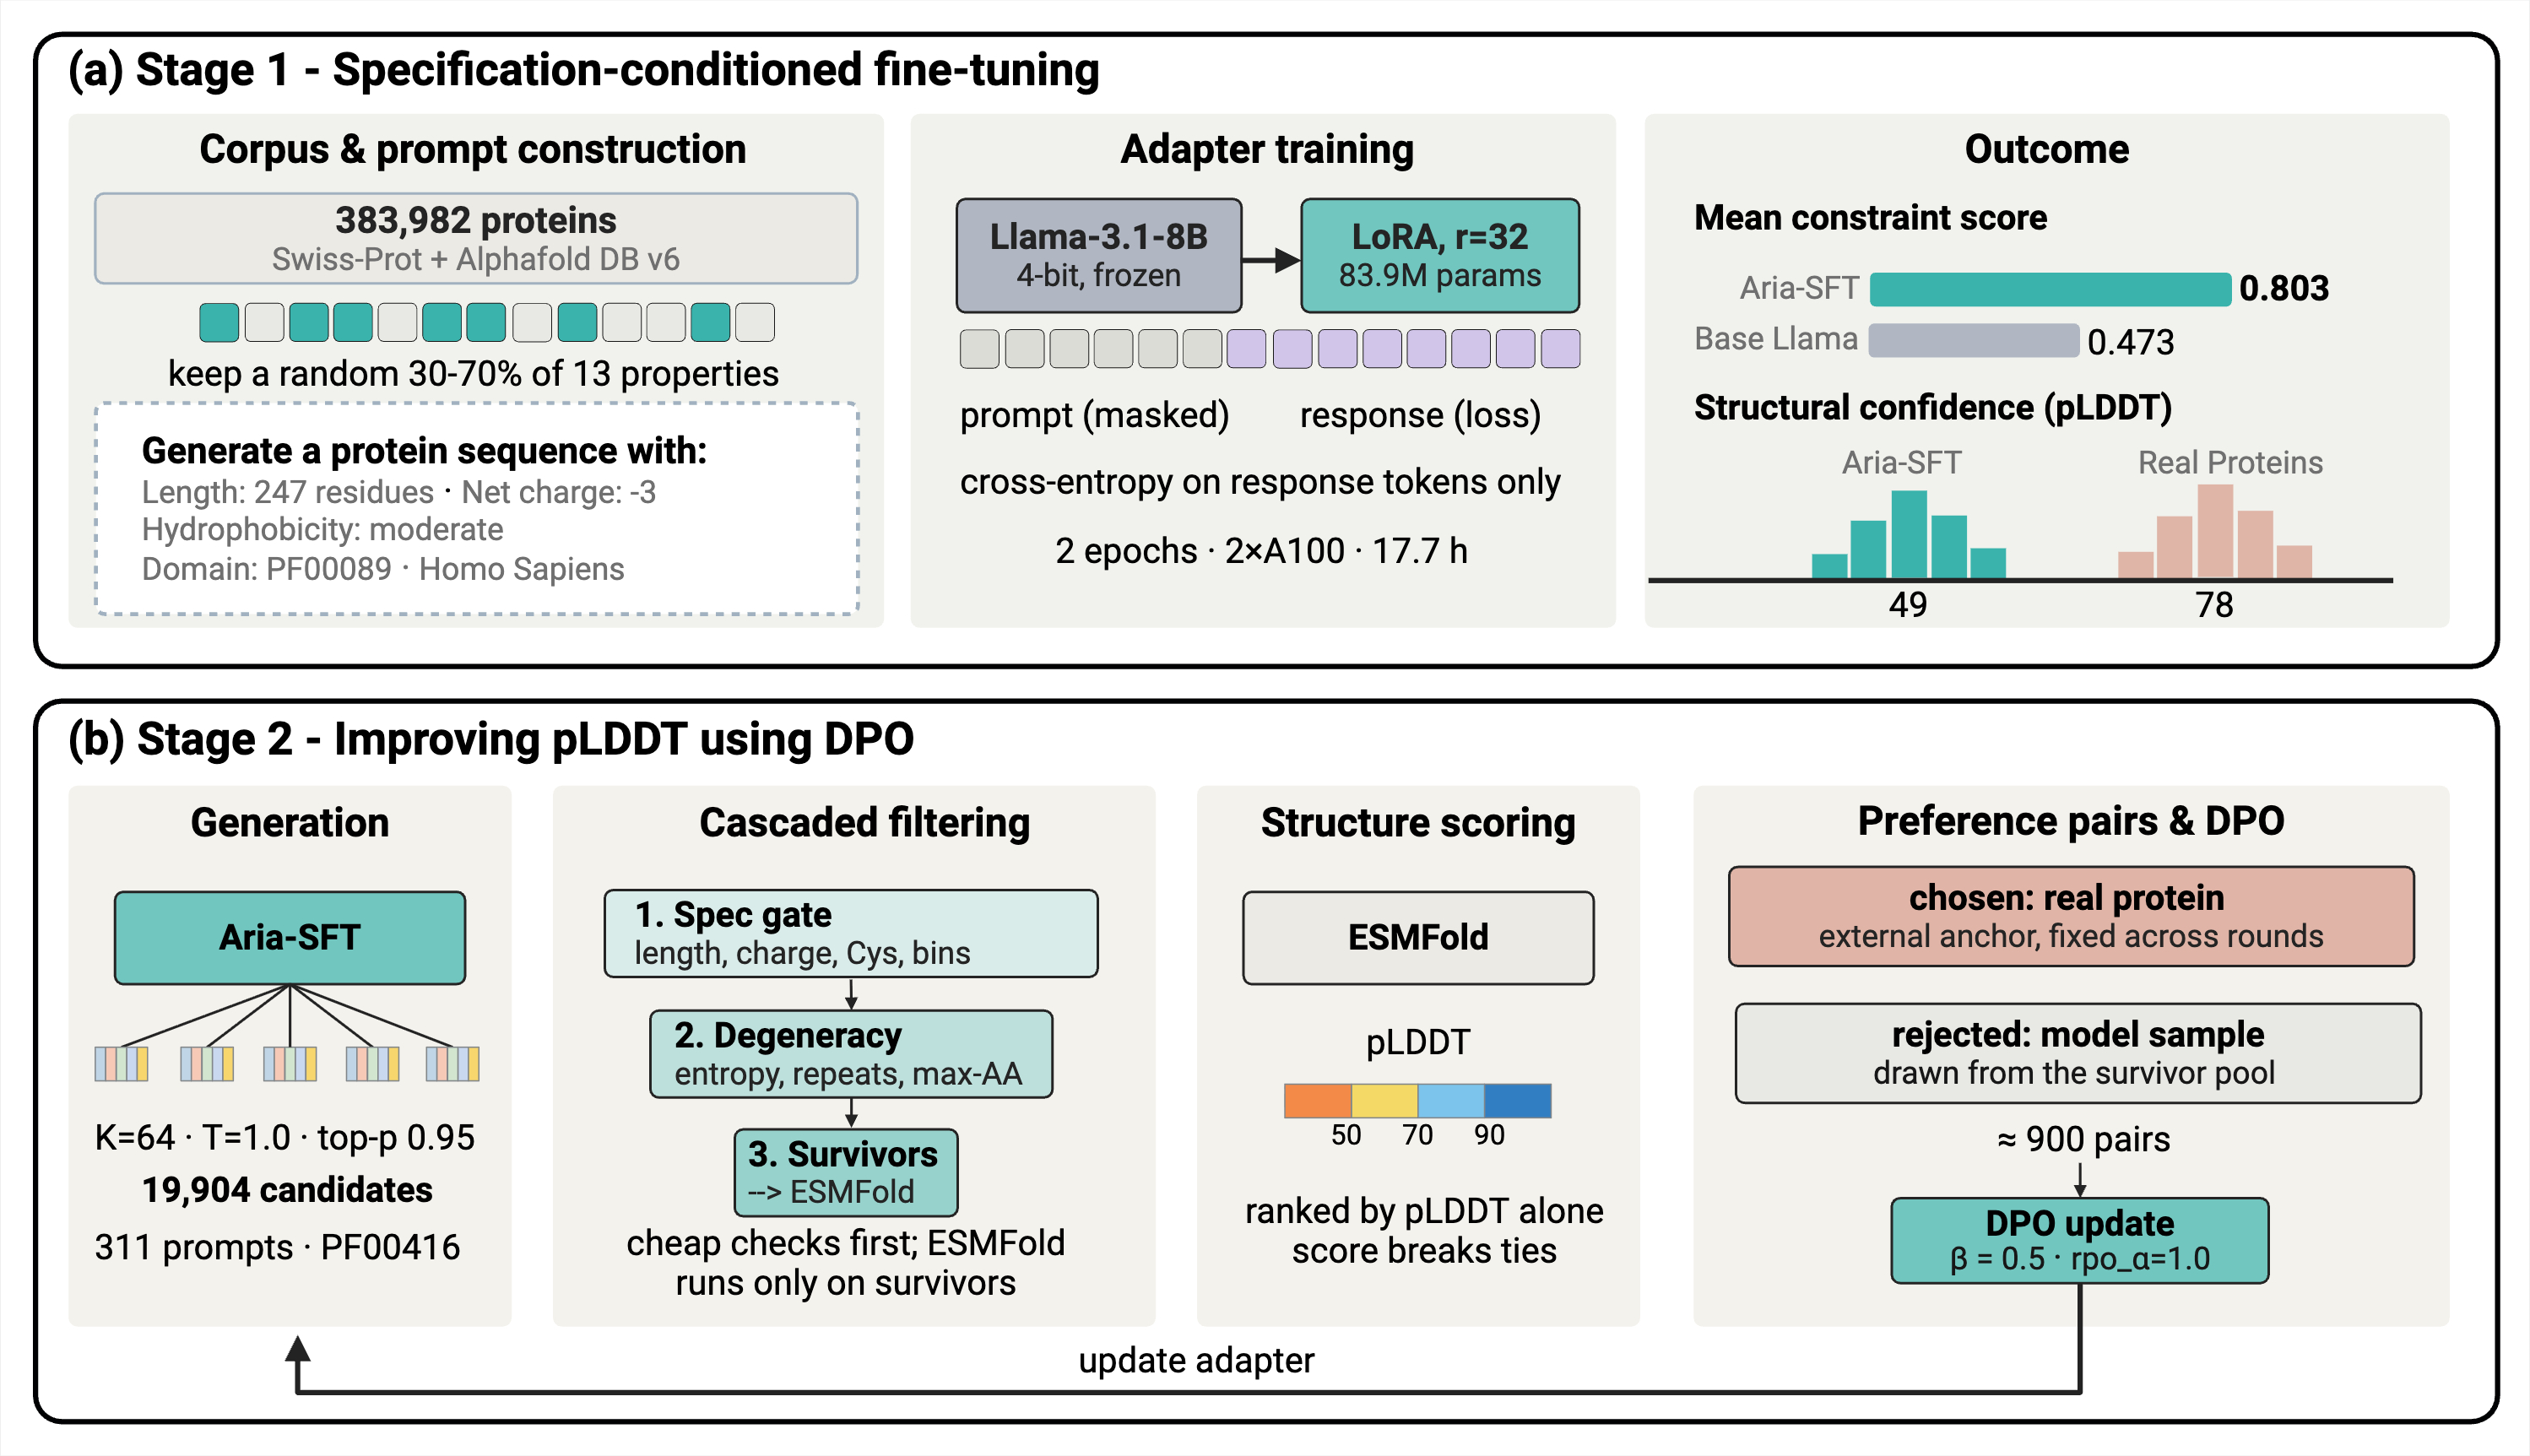
\includegraphics[width=\linewidth]{figures/Fig1_V2.jpeg}
  \caption{The Aria training and preference-optimization workflow.
  (a) During specification-conditioned fine-tuning, each example pairs
  a specification containing a randomly selected 30-70\pct{} subset of thirteen
  protein descriptors with its natural sequence; loss is computed only over the
  sequence. (b) Preference optimization against that measure, shown for ribosomal protein uS13
(PF00416) and applied identically to three further Pfam families. Candidates
sampled from the supervised model pass a specification gate and composition
filters before structure prediction, so ESMFold is run only on survivors. For
each prompt the natural Swiss-Prot sequence supplies the preferred response and
a surviving generation the rejected one, fixing one side of every comparison at
a point that satisfies the specification by construction. The adapter is updated
and the loop repeats for up to three rounds.} \label{fig:pipeline}
\end{figure}
Protein language models have made sequence generation routine. Autoregressive
models trained on large sequence corpora, among them ProGen
\citep{madani2023progen}, ProGen2 \citep{nijkamp2023progen2} and ProtGPT2
\citep{ferruz2022protgpt2}, emit sequences that fold and resemble natural
proteins, and encoder families such as ESM \citep{lin2023esm2} represent them
well enough to support structure prediction. Producing a plausible protein is no
longer the difficulty. Directing that production is.

Two obstacles stand in the way, and they compound each other. The first is that the interface is often narrow. For example, 
ProGen and ProGen2 condition on family or keyword tags, ProtGPT2 does not
condition at all, and ProLLaMA \citep{lv2026prollama} exposes a single
categorical axis, the protein superfamily, treating physicochemical properties
as a decode-time filter rather than as targets a user may set. Work that does address attributes directly steers through learned tokens or model-internal interventions \citep{ismail2025cbplm, luo2026prefixprot, liu2025ctrlprot, hayes2025esm3}, or aligns free-text function descriptions with sequence \citep{liu2025proteindt, wang2024instructprotein}, rather than accepting a user-provided textual specification. The second obstacle is measurement. Evaluations across recent protein-generation studies \citep{madani2023progen,nijkamp2023progen2,
ferruz2022protgpt2} are dominated by perplexity, predicted structural confidence \citep{jumper2021alphafold}, and template-modeling scores \citep{zhang2004tmscore}. These metrics ask whether a generation resembles a protein, not whether it carries the properties that were requested. This distinction matters in practice: a model that disregards a stated net charge while emitting a well-folded sequence scores well on commonly used measures, and the failure surfaces only downstream, during purification or formulation.

Instruction tuning can address both at once \citep{zhang2023instructiontuning}. A
general instruction-tuned model already accepts conditions stated in natural
language, so a conjunctive, partial request needs no bespoke interface, only
training data in which such requests appear; and for many properties the request
is verifiable, since the property can be recomputed on the generated sequence
with the function that wrote the specification.

Using this approach, we instruction-tune Llama-3.1-8B-Instruct
\citep{dubey2024llama3} with QLoRA \citep{dettmers2023qlora, hu2022lora} on
348{,}867 Swiss-Prot proteins, each described by a partial, randomly sampled
subset of thirteen physicochemical, developability, structural and functional
descriptors written into the prompt, and evaluate on 35{,}115 held-out
specifications separated from training by sequence clustering. A
single low-rank run of approximately 35 GPU-hours, updating 1\pct{} of the
parameters without protein-specific pre-training, improves adherence on every
axis we can recompute. Composition follows the specification closely: length
within $\pm$10\pct{} rises from 11.6\pct{} to 88.8\pct{} and exact cysteine
count from 23.3\pct{} to 68.9\pct. Topology follows it as well, with
transmembrane-helix Matthews correlation rising from 0.275 to 0.869 and signal
peptide from 0.073 to 0.739. Exact Pfam-domain recovery is the exception, at
2.9\pct, and increases with domain exposure during training.

Adherence, however, is not accompanied by confident structure: mean ESMFold
pLDDT lies between 45 and 59 across the families we examine, against 77 to 83
for their natural members. Because these evaluations are computed from sequence,
they can act as training signals rather than only as scores. We
therefore use the same measure as a reward, applying direct preference
optimization \citep{rafailov2023dpo} anchored on natural family sequences to
four Pfam families. 
Mean pLDDT increases in all four families, with gains reproduced at two
training seeds in the three additional families and reaching up to 13.1 points, closing the distance to natural members of the same family.

In the three additional families, two measures not used to rank preference
pairs improve alongside predicted confidence: recovery of the requested
domain, assessed by hmmsearch against each family's own profile, rises
from 9-44\pct{} to 30-80\pct{}, and the fraction of generations reaching
the natural fold increases in all three families. The gains do not transfer consistently across families. Across six transfer targets, family-specific adapters do not consistently improve requested-domain recovery. Direct preference optimization on three targets nevertheless increases strict-composite passage, indicating that limited cross-family transfer does not preclude improvement using target-family examples.

These results indicate that a general instruction-tuned model can be
repurposed into a specification-conditioned protein generator through a
single parameter-efficient fine-tuning run, and that evaluation-guided
preference optimization can subsequently improve predicted structural
confidence and domain recovery, although its effects on specification
adherence vary across families. Although demonstrated here for a general-use language model, this formulation provides a testable route to improving adherence in existing protein language models.

\section{Results}
\label{gen_inst}
\begin{figure}[b!]
\centering
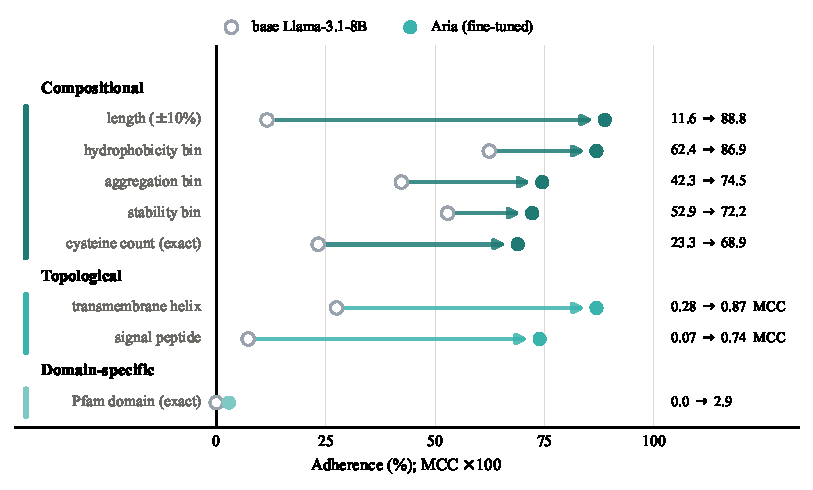
\includegraphics[width=\linewidth]{figures/fig-tiers.pdf}
\caption{The controllability hierarchy. Each row shows adherence for one property before and after supervised
fine-tuning. Open markers denote the base model, filled markers
denote Aria, and connecting lines indicate the change. Rows are read independently, so percentage and MCC rows
share one axis with MCC $\times$100. Enzyme class is omitted because
its measurement is confounded (Appendix~\ref{app:ec}).}
\label{fig:tiers}
\end{figure}

Supervised instruction tuning improves adherence across the evaluated
properties, but the degree of control varies by property class
(Figure~\ref{fig:tiers}, Table~\ref{tab:controls}). Adherence improves for compositional, developability-related (aggregation propensity and cysteine count), and topological properties, and topology show substantial improvements, whereas recovery of the requested protein
family or domain, as represented in the Pfam database, remains low. We first characterize these
differences and evaluate the dependence of adherence on the requested
specification. We then examine whether anchored preference optimization
improves predicted structural confidence and domain recovery, how it
affects specification adherence, and whether the gains transfer across
families.

\paragraph{Tier 1: Composition and Developability.}
Fine-tuning first teaches the model to return the requested output format: the fraction of generations containing a bare sequence rather than prose rises from 0\pct{} to 99.9\pct. Beyond formatting, adherence improves across every measured sequence-derived property. Length adherence rises from 11.6 to 88.8\pct, hydrophobicity from 62.4 to 86.9\pct, and exact cysteine-count adherence from 23.3 to 68.9\pct; aggregation and stability show similar gains (Figure~\ref{fig:tiers}).
While exact numerical control remains less precise for charge, the correlation between requested and realized net charge rises from $r=0.26$ to $r=0.89$, showing that the model responds strongly to the requested direction (Table~\ref{tab:controls}, Appendix~\ref{app:charge}).

\paragraph{Tier 2: Topology.}
Transmembrane-helix recall increases from 14.0\pct{} to 86.5\pct{}, and Matthews correlation coefficient (MCC) from 0.275 to 0.869. Signal-peptide recall increases from 6.6\pct{} to 61.4\pct{}, with MCC rising from 0.073 to 0.739. Positive-class precision remains high at 91.4\pct{} for transmembrane helices and 93.2\pct{} for signal peptides, indicating that the increased recall is accompanied by specificity for the requested topological features (Figure~\ref{fig:tiers}).

\paragraph{Tier 3: Domain Identity.}
Domains are assigned using hmmscan
\citep{eddy2011hmmer} against Pfam-A \citep{mistry2021pfam}, where lower $E$-values indicate stronger evidence for a sequence-profile match. At the default reporting threshold, the requested domain is detected in 2.90\% of fine-tuned generations (520 of 17{,}941), compared with none of 15{,}140 base-model generations. The few highly significant assignments are nevertheless specific: among the 145 generations receiving any match at $E\leq10^{-10}$, 71.0\% match the requested domain. The aggregate recovery rate is partly depressed by uneven training exposure: many requested domains are absent or rare in training, and success increases markedly with their representation (Appendix~\ref{app:domain}, Figure \ref{fig:domain}). Thus, the model acquires targeted signatures for some represented domains, but exact-domain control across the full held-out set remains limited. Whether it can be improved within a single family, using the same recomputed measurements as a training signal, is examined in Section~\ref{sec:dpo}.


\subsection{Adherence reflects prompt conditioning}

\begin{table}[b]
\caption{Prompt-conditioned adherence on directly recomputable properties.
The value of $n$ is the number of valid Aria generations whose specification
requested the corresponding property. Bracketed values are 95\% Wilson
confidence intervals for Aria's adherence rate.\\}
\label{tab:controls}
\centering
\small
\begin{tabular}{lrrrr}
\toprule
Property
    & $n$
    & \textbf{Aria [95\% CI]}
    & Constant
    & Mismatch \\
\midrule
Length ($\pm10\pct$)
    & 19{,}140
    & \textbf{88.8\pct{} [88.4, 89.3]}
    & 19.8\pct
    & 11.9\pct \\
Hydrophobicity bin
    & 19{,}030
    & \textbf{86.9\pct{} [86.4, 87.3]}
    & 72.4\pct
    & 52.3\pct \\
Aggregation bin
    & 18{,}966
    & \textbf{74.5\pct{} [73.9, 75.2]}
    & 34.2\pct
    & 33.0\pct \\
Stability bin
    & 18{,}998
    & \textbf{72.2\pct{} [71.5, 72.8]}
    & 55.0\pct
    & 51.7\pct \\
Cysteine count (exact)
    & 18{,}853
    & \textbf{68.9\pct{} [68.3, 69.6]}
    & 17.5\pct
    & 10.4\pct \\
Net charge ($\pm2$)
    & 18{,}919
    & \textbf{35.2\pct{} [34.5, 35.9]}
    & 25.3\pct
    & 14.9\pct \\
\bottomrule
\end{tabular}
\end{table}

Raw adherence can be inflated by common property values even when a
model ignores the prompt. We therefore compare Aria with two
request-blind controls: a constant baseline that always predicts the
most frequent training value, and a mismatch control that scores each
generated sequence against a different held-out specification. Aria
exceeds both controls on all six directly recomputable properties
(Table~\ref{tab:controls}). Mismatching specifications reduces adherence
by between 20.3 percentage points for net charge and 76.9 percentage
points for length. Mean compositional adherence also remains similar
when the requested Pfam family is absent from training
(71.4\pct{}, compared with 71.0\pct{} for represented families). Thus, the model can follow compositional requirements even when the requested family was not represented during fine-tuning.
Together, these findings support dependence on the requested
specification and indicate that compositional control extends to
proteins from families absent from supervised training.

\subsection{Additional constraints do not weaken length control}

We next test whether adding other requested properties weakens control of a fixed length target. For this experiment, we use a subset of 200 proteins from the cluster-separated held-out set. For each protein, we construct thirteen nested specifications, starting with length alone and adding one descriptor at each step while keeping the requested length unchanged. Length adherence remains between 84 and 92\%, with no significant trend as constraints are added (slope $+0.028$, 95\% CI $[-0.006,+0.061]$; Appendix~\ref{app:ladder}). Thus, length adherence remains stable across the tested constraint ladder.

\subsection{Anchored DPO improves predicted structural confidence
and domain recovery}
\label{sec:dpo}

Supervised tuning improves compositional and topological control, but requested-domain recovery remains limited and predicted structural confidence falls below that of natural family members. We therefore seek to shift the generation distribution towards sequences with higher predicted structural confidence and stronger family-specific characteristics while retaining specification adherence. To this end, we apply natural-sequence-anchored direct preference optimization (DPO) as a post-training stage, which increases the relative likelihood of preferred natural sequences over generated alternatives \citep{rafailov2023dpo}. 

We construct preference pairs using ESMFold pLDDT as the structural-confidence criterion. Before structure prediction, a specification gate checks agreement with the requested sequence-derived properties, while sequence filters exclude low-complexity, excessively repetitive, or compositionally imbalanced outputs. Candidates passing both checks (gate and filter) are folded with ESMFold and paired with the matching natural sequence when its predicted confidence is higher. The natural sequence serves as the preferred response. Training combines DPO with an auxiliary negative-log-likelihood term on preferred responses \citep{pang2024rpo}. This configuration mitigated the reward-hacking failure observed
under self-play preferences, in which higher ESMFold confidence was accompanied by poorer specification adherence and sequence composition (Appendix~\ref{app:selfplay}, Figure~\ref{fig:reward-hacking-example}). Domain recovery and structural similarity are evaluated separately and are not used to construct the preference ordering.

We first evaluate this approach on ribosomal protein uS13 (PF00416), using 311 natural sequences for preference construction and 260 cluster-separated sequences for held-out evaluation. Pairing the training sequences with eligible generated candidates yields 929 preference pairs, because a natural sequence can be paired with more than one candidate. One training stage increases mean ESMFold pLDDT from 49.4 to 57.6, compared with 78.0 for the full natural reference set of 571 sequences (311 training and 260 held-out). Under matched evaluation with one generation per model per prompt, specification-gate passage increases from 16.9\pct{} to 25.8\pct{} and sequence-filter passage from 88.5\pct{} to 96.5\pct{}. The strict composite requiring the gate, filters, and pLDDT $\geq70$ increases from 0.4\pct{} to 7.3\pct{}
(1 to 19 of 260 prompts). Thus, predicted confidence and these population-level adherence measures improve concurrently in PF00416.

To assess whether the improvements extend beyond PF00416, we repeat anchored preference optimization on three additional families: ribosomal proteins uL22 (PF00237) and uL24 (PF00467), and YqgF (PF03652). Each undergoes three rounds of anchored preference
optimization at two training seeds, with separate preference-training, validation, and final-test splits. Evaluation uses one generation per held-out prompt; outputs without an extractable sequence count as
failures in population pass rates. Mean pLDDT increases relative to the supervised model in all three groups at both seeds.

To assess whether the confidence gains are accompanied by improvements beyond the preference-selection metric, we also measure requested-domain recovery and structural similarity to the corresponding natural references. Both improve, although neither is used to rank preference pairs. Here,
domain recovery is assessed using hmmsearch against the requested
Pfam profile with its curated gathering threshold, rather than the
full Pfam-A scan used in the broad supervised evaluation. At the
checkpoints used for subsequent transfer experiments (round two for
PF00237 and round three for PF00467 and PF03652) domain recovery averaged across the two seeds increases from 9.0\pct{} to 29.8\pct{}, 28.4\pct{} to 72.0\pct{}, and 44.2\pct{} to 80.0\pct{}, respectively. The fraction of generations whose predicted structures achieve TM-score $\geq0.5$ against the corresponding natural-reference
structures also increases in all three groups at both seeds (Figure~\ref{fig:families}).

These gains are not accompanied by uniform improvements in
specification adherence. For example, the first PF00237 round
increases mean pLDDT at both seeds, while gate passage decreases
from 40.4\pct{} to 33.7\pct{} at one seed and increases from
28.1\pct{} to 46.1\pct{} at the other. Anchored preference
optimization therefore improves predicted structural confidence
and domain recovery across the tested groups, but preservation
of specification adherence must be assessed separately.

\begin{figure}[t]
\centering
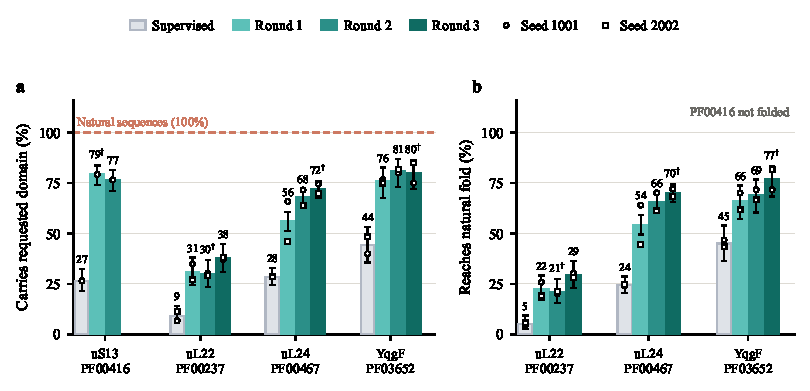
\includegraphics[width=\linewidth]
{figures/fig3-families.pdf}
\caption{Within-family outcomes of anchored preference optimization
for two seeds. (a) Requested-domain recovery.
(b) Fraction of generations with TM-score $\geq0.5$ against the
predicted structure of the corresponding natural reference.
Rates use all held-out prompts as denominators:
260 for PF00416, 89 for PF00237, 211 for PF00467, and 60 for PF03652. Bars show rates averaged across the two seeds and the markers show seed-specific rates.
Error bars show 95\% Wilson intervals and do not represent variation
across training seeds. PF00416 has two optimization rounds and no
TM-score analysis in this comparison. Domain recovery and structural
similarity improve relative to supervised tuning, with trajectories
that vary across families.}
\label{fig:families}
\end{figure}

\subsection{Comparison with a protein-specific language model}

We next assess how supervised Aria compares with a model built specifically
for protein generation, before any family-specific preference optimization.
ProLLaMA \citep{lv2026prollama} is pretrained on protein sequences and
instruction-tuned for superfamily-conditioned generation. Its generation
interface takes one instruction, [Generate by superfamily] Superfamily=name, with the name drawn from the fixed vocabulary the model was trained on. It has no field for length, net charge, hydrophobicity, cysteine count, or any other property target, so the specifications used throughout this paper cannot be presented to it at all. The asymmetry in the
inputs is a property of the baseline rather than a choice in the protocol.
That vocabulary also fixes the scope of the comparison: five of the nine
families in this study have an entry, three have none, and one is represented
only by a different paralog of the same protein.

Each model therefore receives what its interface accepts, Aria the held-out
textual specification and ProLLaMA the corresponding superfamily label. Both
generate one sequence per evaluation case at a sampling temperature of 0.7,
and both are scored against the same criteria.


ProLLaMA achieves higher requested-domain recovery than
supervised Aria in three of the five families
(Table~\ref{tab:prollama}). For example, recovery reaches
96.4\pct{} for ProLLaMA versus 50.0\pct{} for Aria on
PF00886, although this comparison comprises only 28 held-out
cases. Conversely, Aria achieves higher recovery on PF00177
(38.6\pct{} versus 0.3\pct{}), while neither model recovers
PF01157. Domain recovery therefore varies substantially
across families for both models.

Aria passes the specification gate more frequently in all five families, with rates of 28.6-40.4\%, compared with 9.0-16.0\% for ProLLaMA. Aria also achieves higher rates on the strict composite requiring gate passage, sequence-filter passage, and pLDDT $\geq70$ in every family. For ProLLaMA, passing the gate means that a generated sequence happens to meet property targets that were not supplied to the model; it does not measure its ability to follow those targets. The comparison therefore shows a practical distinction between generating a member of a requested family and generating a sequence that also meets additional requirements. With supervised adaptation on 348{,}867 proteins and no protein-specific pretraining, Aria supports multi-property conditioning and achieves higher gate and composite rates in this evaluation, although ProLLaMA recovers the requested domain more frequently in three of the five families.

\begin{table}[t]
\caption{Supervised Aria and ProLLaMA on five evaluated families
covered by ProLLaMA's conditioning vocabulary.  All rates are percentages over the $n$ evaluation cases. The strict composite requires gate passage, sequence-filter passage, and pLDDT $\geq70$.\\}
\label{tab:prollama}
\centering
\small
\setlength{\tabcolsep}{3pt}
\begin{tabular}{@{}lr*{6}{r}@{}}
\toprule
 & & \multicolumn{2}{c}{Domain recovery}
   & \multicolumn{2}{c}{Gate passage}
   & \multicolumn{2}{c}{Strict composite} \\
\cmidrule(lr){3-4}
\cmidrule(lr){5-6}
\cmidrule(lr){7-8}
Family & $n$
 & ProLLaMA & Aria
 & ProLLaMA & Aria
 & ProLLaMA & Aria \\
\midrule
PF00237 & 89
 & 29.2 & 6.7 & 9.0 & 40.4 & 1.1 & 9.0 \\
PF00177 & 352
 & 0.3 & 38.6 & 10.5 & 33.5 & 0.0 & 4.8 \\
PF01196 & 168
 & 57.7 & 50.6 & 10.7 & 28.6 & 0.6 & 11.9 \\
PF00886 & 28
 & 96.4 & 50.0 & 10.7 & 39.3 & 10.7 & 25.0 \\
PF01157 & 50
 & 0.0 & 0.0 & 16.0 & 40.0 & 0.0 & 8.0 \\
\bottomrule
\end{tabular}
\end{table}

\subsection{Preference optimization does not consistently transfer
across families}
The within-family improvements raise the question of whether an adapter optimized on one family can benefit other families without constructing new preference pairs for each target. We test this using the adapters trained separately on the three additional families in Section~\ref{sec:dpo}, treating these as source families. Six other families, selected for proximity to a source in the family-level ESM2 embedding, serve as transfer targets and contribute no examples to source-family preference training. Each target is evaluated with all three source adapters at both training seeds, yielding 18 source-target combinations per seed. We compare each adapter with the supervised model on the same held-out target specifications (Figure~\ref{fig:transfer}).
\begin{figure}[h]
\centering 
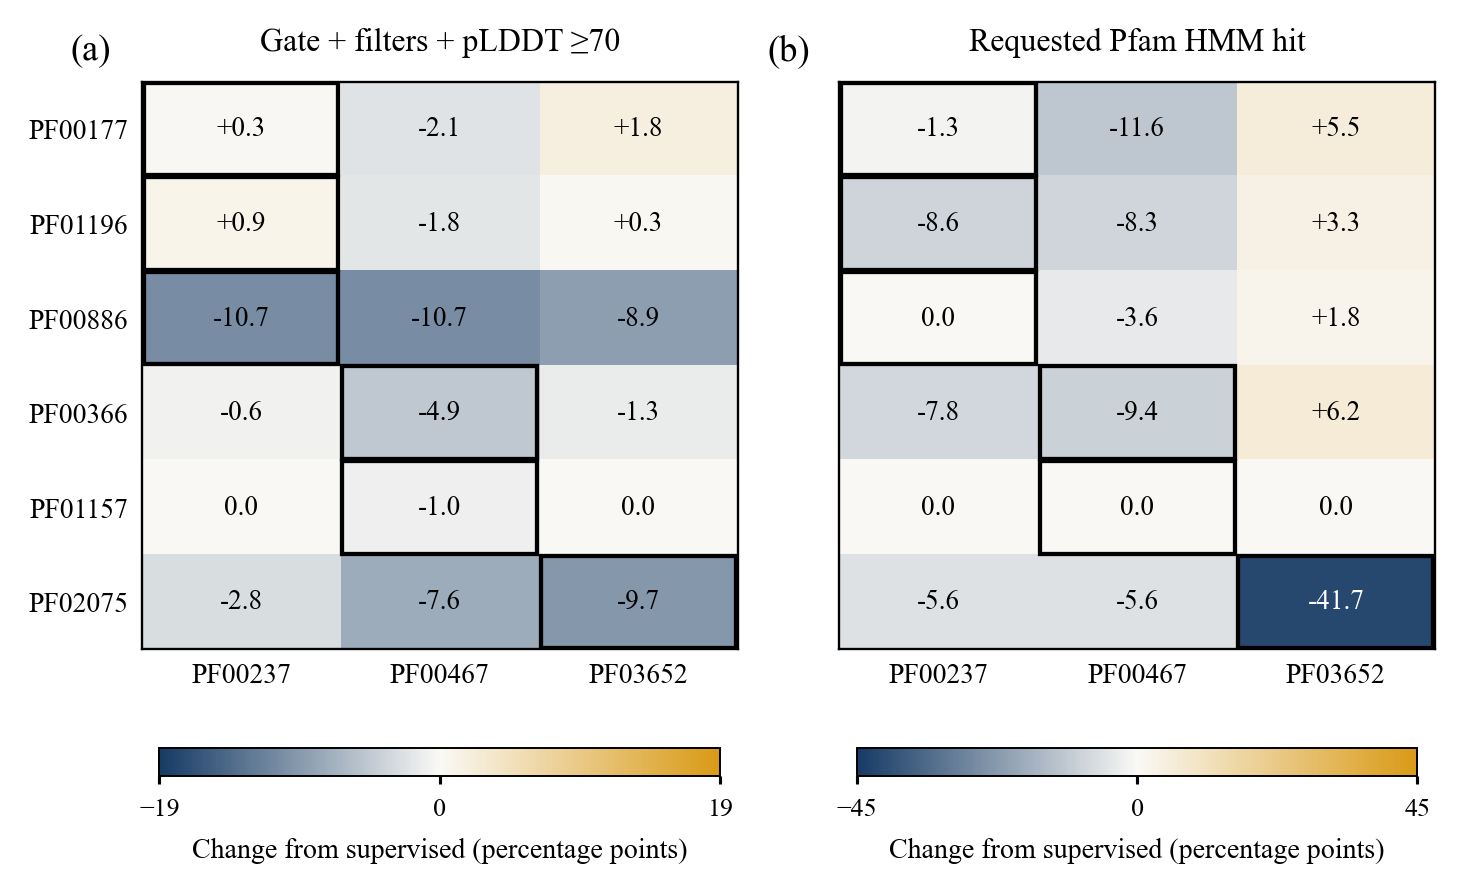
\includegraphics[width=0.82\linewidth]
{figures/heatmap_deep_navy_amber.png}
\caption{Transfer of family-specific preference optimization. Columns identify source families used for preference training; rows identify target families excluded from that training. Cells show changes from the corresponding supervised baseline, averaged across two seeds, in percentage points. (a) Strict-composite passage, requiring the specification gate, sequence filters, and pLDDT $\geq70$. (b) Requested-domain recovery. Black outlines identify preassigned nearby source-target pairs. The adapters are from round two for PF00237 and round three for PF00467 and PF03652.}
\label{fig:transfer}
\end{figure}

Transfer is heterogeneous and does not reproduce the consistent within-family improvements. Averaged across seeds, requested-domain recovery decreases for four of the six preassigned nearby source-target pairs and remains unchanged for two. The strict composite requiring specification-gate passage, sequence-filter passage, and pLDDT $\geq70$ decreases in 25 of the 36 source-target-seed comparisons. An increase in domain recovery does not necessarily imply an increase in strict-composite passage. For example, the PF03652 adapter increases domain recovery on PF00366 by 6.2 percentage points averaged across seeds, while the strict-composite rate decreases by 1.3 points.

To separate the contribution of a transferred adapter from that of the target family's own preference data, we optimized three of the six target families directly, each from two starting points, with two runs per configuration. Ribosomal proteins bL17 (PF01196) and uS17 (PF00366), and the RuvC family (PF02075), each
received three anchored rounds beginning either from the general supervised
model or from the adapter trained on that target's nearest source family. All
other settings match Section~\ref{sec:dpo}, and both conditions use the target's
own preference-training split.

The two conditions begin far apart. Averaged across seeds, requested-domain
recovery at the starting checkpoint is 55\pct{} for the supervised model against
43\pct{} for the transferred adapter on PF01196, 23\pct{} against 14\pct{} on
PF00366, and 68\pct{} against 35\pct{} on PF02075. This restates the transfer
result above in a third form: the adapter optimized on the nearest source is a
worse starting point than the model it was derived from.

Target-family preference optimization increased requested-domain recovery from both the general supervised and nearby-family initializations (Figure~\ref{fig:warmcold}). We compare the two initializations after three rounds of optimization. Strict-composite passage on PF01196 reached 21.4-23.8\% from the general supervised initialization and 22.6-24.4\% from the nearby-family initialization. Corresponding rates were 26.6-27.9\% and 20.8-24.7\% on PF00366, and 29.2-30.6\% and 22.2-23.6\% on PF02075. Ranges describe the two runs, not confidence intervals.

\begin{figure}[h]
\centering
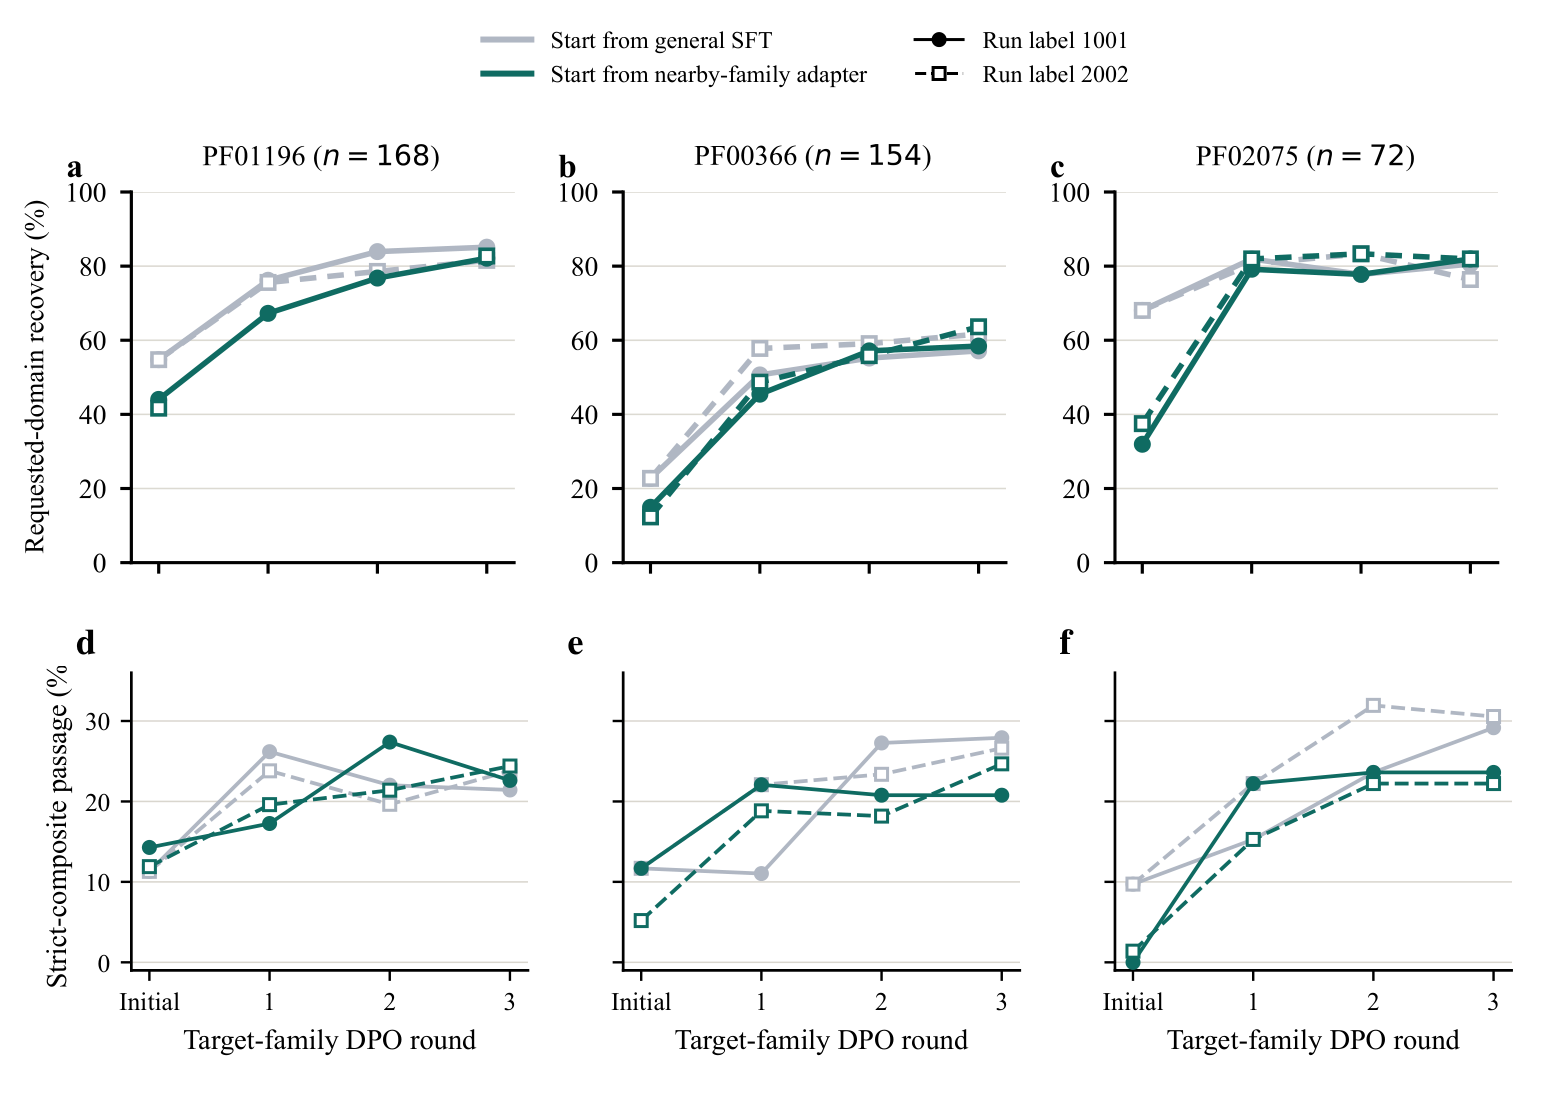
\includegraphics[width=0.85\linewidth]{figures/figure5_two_rows_updated.png}
\caption{Starting point against destination for three families that also serve
as transfer targets. (a-c) Requested-domain recovery, assessed with hmmsearch against the family's own Pfam profile.
(d-f) Strict-composite passage, requiring the specification gate, the
sequence filters, and pLDDT $\geq70$. The initial point is the checkpoint each
condition began from, so the nearby-family series starts at the transferred
adapter's rate rather than the supervised model's. Rates are over all held-out
prompts.}
\label{fig:warmcold}
\end{figure}

These results distinguish cross-family transfer from optimization using target-family examples. Target-family optimization improved strict-composite passage across all three tested families, whereas initialization from a nearby-family adapter did not yield consistently higher round-three rates than initialization from general supervised Aria.

\section{Discussion}
Across the tested axes, Aria shows a hierarchy of controllability. Gains are strongest for physicochemical, developability, and topological properties, whereas exact Pfam-domain recovery remains low in the broad supervised evaluation. Request-blind controls show that the composition gains are not explained solely by an unconditional shift in model outputs. On cluster-separated evaluation proteins, composition control persists, whereas exact domain recovery increases with family exposure (Appendix~\ref{app:domain}). Controllability therefore depends on both the requested property and, for domain identity, training exposure. On PF00416, one natural-sequence-anchored DPO stage raises mean ESMFold pLDDT from 49.4 to 57.6 and improves the property gate, sequence filters, and strict composite under matched one-sample evaluation. Nevertheless, 57.6 remains below the ESMFold mean of 78.0 for the natural PF00416 reference set. One round therefore closes approximately 29\% of this confidence gap, yielding a substantial but partial improvement.

The additional experiments extend these findings beyond PF00416: predicted structural confidence, requested-domain recovery, and structural similarity improve across three further families at both training seeds. However, specification adherence does not improve uniformly, and the resulting adapters do not consistently benefit other families. Direct preference optimization increases strict-composite passage across three target families, whereas the available cold- and warm-start comparisons do not establish a consistent benefit from nearby-family initialization. These findings support target-specific adaptation rather than assuming that improvements learned within one family will transfer to another. The ProLLaMA comparison further distinguishes domain recovery from multi-property adherence: neither model dominates domain recovery across families, whereas Aria achieves higher specification-gate and composite rates under its richer conditioning interface.

Several limitations remain. Supervised adaptation was evaluated with one training run of an 8B model. The preference-optimization experiments cover a restricted set of families and a limited number of runs, leaving variability across model scales and broader biological settings uncharacterized. ProLLaMA has no interface for property targets, so that comparison cannot be run under exact identical inputs and does not isolate the effect of the training procedures. Moreover, anchored preference optimization requires matching natural sequences as preferred responses; its applicability to specifications without such examples remains untested. All structural and functional assessments are computational: increased ESMFold confidence, structural similarity, and Pfam-profile recovery do not establish experimental folding or biological function. 

Within these bounds, the study demonstrates a parameter-efficient route to multi-objective, property-conditioned protein generation. More broadly, the measurement-to-feedback strategy may improve adherence in an existing protein generator whenever the requested property can be reliably evaluated.


\subsection*{AI use statement}

We used generative AI assistance to discuss and refine experimental methodology, interpret results, and identify limitations and potential confounders. AI tools also assisted with literature searches, drafting and revising manuscript text, implementation and debugging of training and evaluation pipelines, analysis code, and scientific visualizations. The authors reviewed and revised the AI-assisted text and figure designs. AI assistance was not used to create an additional synthetic protein dataset; model-generated sequences used in the experiments, including preference construction, are described in the Methods. The authors are responsible for the final manuscript, including its analyses, citations, claims, and AI-assisted artifacts.

\subsection*{Reproducibility statement}

Details sufficient to reproduce the reported results are given in the appendices. Appendix~\ref{app:method} specifies the base model, the adapter configuration, the optimization settings, the construction of preference pairs, and the evaluation procedure, including the criteria applied by the specification gate and the sequence filters. Appendix~\ref{app:desc} lists the thirteen conditioning descriptors, their
sources, and the methods used to evaluate adherence. Appendix~\ref{app:compute} reports the training footprint, and Appendix~\ref{app:clustering} states the rule by which source and target families were selected, which was fixed before any preference training. Corpus construction, the cluster-level separation of training from evaluation sequences, and the disjoint preference-training, validation and test partitions within each family are described in Appendix~\ref{app:method}; reported checkpoints were selected on the validation split, and the test split was not consulted during selection. External tools are applied at published settings: ESMFold for structure prediction, HMMER with Pfam gathering thresholds for domain assignment, and TM-score for structural comparison. The three families optimized after PF00416 were each trained at two seeds.


\bibliography{iclr2027_conference}
\bibliographystyle{iclr2027_conference}

\appendix
\setcounter{figure}{0}
\renewcommand{\thefigure}{A\arabic{figure}}
\setcounter{table}{0}
\renewcommand{\thetable}{A\arabic{table}}

\section{Method}\label{app:method}


Aria is built in two stages (Figure~\ref{fig:pipeline}). 

\paragraph{Corpus and specifications.} From the reviewed subset of UniProt
\citep{uniprot2023} we keep sequences of 20-512 residues with canonical
residues, no fragments and no duplicates, leaving $\sim$384k proteins. To
prevent leakage we cluster with MMseqs2 \citep{steinegger2017mmseqs2} at
30\pct{} identity and 80\pct{} coverage and split at the \emph{cluster} level:
348{,}867 training and 35{,}115 held-out proteins, no held-out protein above
30\pct{} identity to any training protein. Thirteen descriptors span four
families (Appendix~\ref{app:desc}): physicochemical and developability
properties computed from the sequence with Biopython \citep{cock2009biopython}
and an AGGRESCAN scale \citep{conchillosole2007aggrescan}; structural and
topological properties from AlphaFold \citep{jumper2021alphafold} and UniProt
annotations; and curator-assigned functional annotations. Each specification
contains a random 30-70\pct{} subset of the descriptors a protein has (3-10
per prompt, mean 6.6), which trains the model for the realistic
under-specified case. The target completion is the bare sequence.

\paragraph{Training.} QLoRA \citep{dettmers2023qlora, hu2022lora} on
Llama-3.1-8B-Instruct \citep{dubey2024llama3}: 4-bit base, rank-32 adapter
($\alpha=16$), two epochs, loss on the completion only. 83.9M trainable
parameters, $\sim$35 GPU-hours. No protein-specific pre-training.

\paragraph{Evaluation.} Adherence is computed only over specifications that
requested a property, so $n$ varies per property. Six axes are recomputed with
the feature code that built the prompt; applying it to the reference Swiss-Prot
sequence returns 100\pct{} by construction, which bounds definitional slack at
zero. Signal peptides use SignalP~6 \citep{teufel2022signalp6}, transmembrane
helices DeepTMHMM \citep{hallgren2022deeptmhmm}, domains \texttt{hmmscan}
\citep{eddy2011hmmer} against Pfam-A \citep{mistry2021pfam}. We report MCC for
the imbalanced binary topology tasks. GO and organism are not scored. The base
model is prompted identically; it embeds sequences in prose, so we extract the
longest canonical residue run, and outputs with none are dropped from
denominators rather than counted as failures, which favours the baseline.

\paragraph{Multi-family study and data partitioning.}
We extended preference optimisation to three source families:
PF00237, PF00467, and PF03652. The original cluster-separated
supervised test partition was retained for final evaluation.
Within the supervised training partition, clusters were further
divided into preference-training and validation subsets.
Validation therefore excluded preference-training examples,
but was not held out from the preceding supervised training.
The resulting preference-training/validation/test counts were
502/111/89 for PF00237, 342/67/211 for PF00467, and
316/71/60 for PF03652.

\paragraph{Source and transfer-target selection.}
We represented 2,403 Pfam families with at least 20 sequences
using mean ESM-2 sequence embeddings and grouped their normalised
representations into 600 clusters. Source selection considered
cluster medoids representing soluble proteins of 80-200 residues,
with at least 250 preference-training, 20 validation, and 20 test
examples, and mean annotated AlphaFold confidence of at least 70.
Among qualifying sources with eligible transfer targets, we
selected three in descending order of cluster size.
Transfer targets were nearby families within the corresponding
embedding cluster, subject to the same length, solubility, and
confidence criteria and at least 20 test examples; no minimum
preference-training count was required.
The six targets were PF00177, PF01196, PF00886, PF00366,
PF01157, and PF02075, with 352, 168, 28, 154, 50, and 72
test prompts, respectively. These families were excluded from
source-family preference optimisation, but not necessarily
from the original supervised training corpus.

\paragraph{Iterative natural-sequence-anchored preference optimisation.}
For each source family, we performed three optimisation rounds
with seeds 1001 and 2002. Each round sampled 64 candidates per
preference-training prompt from the current adapter. Candidates
were screened by the specification gate and sequence filters
before ESMFold evaluation. The matching natural sequence served
as the preferred response, and eligible generated sequences
served as rejected responses when their mean pLDDT was at least
five points lower than that of the natural sequence. Up to
three rejected responses were retained per prompt, selecting
the lowest-confidence eligible candidates.

Each round continued from the preceding adapter, while the
reference policy remained the original supervised model.
Training used the sigmoid DPO objective with $\beta=0.5$ and
an additional preferred-response negative-log-likelihood term
with coefficient 1.0. The recorded configuration used
rank-32 LoRA adapters with scaling parameter 16 and dropout
0.05, a learning rate of $5\times10^{-5}$, an effective batch
size of eight, and 60 optimisation steps per round.
Accordingly, this experiment evaluates anchored preference
optimisation with a supervised auxiliary term, rather than
an unregularised DPO objective.

\paragraph{Specification gate.}
The gate evaluates the requested sequence-derived properties and requires a valid amino-acid sequence. Requested length must be within $\pm10\%$ of its target and net charge within $\pm2$ charge units. Cysteine counts must match exactly for targets of zero, one, or two; larger targets allow a deviation of one residue. Stability bins must match exactly. For hydrophobicity and aggregation, an adjacent ordinal bin is permitted, but a low-high mismatch is rejected. The gate additionally requires an aggregate constraint score of at least 0.70. These criteria differ from the exact-bin and exact-cysteine adherence measures used in the broad supervised evaluation. Gate passage therefore does not mean exact agreement with every requested descriptor.

\paragraph{Sequence filters.}
Sequence filters require at least 20 canonical amino-acid residues, an amino-acid Shannon entropy of at least 3.2 bits, and no individual residue type comprising more than 23\% of the sequence. The longest contiguous tandem-repeat region, considering repeat periods of one to five residues, must cover no more than 25\% of the sequence. These filters screen for low complexity, residue overrepresentation, and short-period repetition; they do not establish biological function or experimental foldability.

\paragraph{Population-level evaluation.}
Evaluation used one generated response per held-out prompt, without best-of-$k$ selection. We separately measured specification-gate passage, sequence-filter passage, their conjunction, and the fraction reaching ESMFold pLDDT $\geq70$. The strict composite required gate passage, filter passage, and this confidence threshold simultaneously; it did not additionally require a Pfam-domain hit. Binary population rates used all assigned prompts as the denominator, with missing or unsuccessful predictions not counted as successes. Mean pLDDT was calculated over responses with an available confidence estimate. ESMFold confidence was interpreted as a prediction-confidence measure, not as experimental evidence of folding or function.

\paragraph{Domain recovery and structural similarity.}
For the family-specific experiments, requested-domain recovery
was assessed with HMMER using the requested Pfam profile and
its curated gathering threshold (\texttt{--cut\_ga}).
This criterion differs from the $E$-value threshold analysis
used in the broad supervised-generation benchmark.
For the structural comparisons, generated and accession-matched
natural sequences were predicted with ESMFold. Their
C$\alpha$ coordinates were aligned using TM-align through
\texttt{tmtools}, with TM-score normalised by the natural
reference length. We report the fraction of all test prompts
with TM-score $\geq0.5$ as a thresholded structural-similarity
measure; comparisons without an available alignment did not
count as successes.

\paragraph{Cross-family transfer and direct training.}
Each source-family adapter was evaluated on all six transfer targets. The transfer analysis used round 2 for PF00237 and round 3 for PF00467 and PF03652, retaining these checkpoints across both seeds. Heatmap entries report the mean of the two seed-specific percentage-point changes relative to the supervised baseline. The designated nearby source-target pairs were determined from the family embedding, rather than from observed transfer performance.

We compared target-family preference optimization from general
supervised Aria (cold start) and from a nearby-family adapter
(warm start) on PF01196, PF00366, and PF02075.
Preference-training/validation/test counts were 269/115/168,
284/69/154, and 283/78/72, respectively. Warm starts used
PF00237 round two, PF00467 round three, and PF03652 round three,
respectively. Each configuration underwent three optimization rounds
using the target family's natural sequences as preferred responses,
with two runs per configuration. The DPO reference remained fixed
at general supervised Aria for cold starts and at the initial
nearby-family adapter for warm starts. The preference objective and
optimization settings otherwise followed those described above.
Evaluation used one generation per held-out prompt, and endpoint
comparisons used round three for both configurations.

\paragraph{Protein-language-model comparison.}
ProLLaMA was evaluated through its only generation interface,
[Generate by superfamily] Superfamily=$<$name$>$, using the superfamily strings shipped with the model. Families were mapped to that vocabulary on an exact match only, checked against the model's own {superfamilies.txt}: PF00467, PF03652 and PF02075 have no entry, and PF00366 appears only as the eukaryotic eS17 paralog rather than the bacterial uS17 requested here, so all four were excluded rather than substituted with a near neighbour. Generation used the decoding settings from ProLLaMA's own inference script, with the temperature raised from its default of 0.2 to the 0.7 used for Aria throughout, so that neither model is sampled more conservatively than the other. One sequence was generated per evaluation case. Sequences were folded with the same ESMFold model and scored with the same family evaluators as Aria's. Because the property targets cannot be supplied through this interface, ProLLaMA's gate and composite rates measure incidental agreement with those targets rather than an ability to follow them.

\paragraph{Uncertainty.}
Where shown for individual population rates, error bars represent 95\% Wilson binomial confidence intervals. These intervals describe uncertainty across evaluated prompts and do not estimate variability across training seeds. Two-seed heatmap averages are descriptive summaries; their signs alone do not establish statistical significance. 

\section{Descriptors}\label{app:desc}
Thirteen descriptors, with how each specification value is obtained and how
adherence to it is measured. ``Presence'' is the fraction of held-out
specifications in which a descriptor appears, a consequence of partial sampling.
Every value is computational; no descriptor is experimentally measured.


\begin{table}[h]
\caption{Descriptors used for specification conditioning and adherence
evaluation. Presence denotes the percentage of held-out specifications
containing each descriptor.}
\label{tab:descriptors}
\centering
\footnotesize
\begin{tabular}{lllll}
\toprule
Descriptor & Type & Presence & Specified from & Adherence scored by \\
\midrule
\multicolumn{5}{l}{\emph{Physicochemical}}\\
\quad Length                  & exact integer & 54.6\pct & len(seq)   & same function \\
\quad Net charge (pH 7.4)     & exact integer & 53.9\pct & Biopython           & same function \\
\quad Hydrophobicity (GRAVY)  & 3 levels      & 54.3\pct & Biopython           & same function \\
\quad Stability               & 2 levels      & 54.2\pct & Biopython           & same function \\
\addlinespace
\multicolumn{5}{l}{\emph{Developability}}\\
\quad Aggregation propensity  & 3 levels      & 54.1\pct & AGGRESCAN scale     & same function \\
\quad Cysteine count          & exact integer & 53.8\pct & count(C)   & same function \\
\addlinespace
\multicolumn{5}{l}{\emph{Structural and topological}}\\
\quad Structural confidence   & 4 levels      & 52.8\pct & AlphaFold DB        & not scored \\
\quad Transmembrane helix     & binary        & 54.2\pct & UniProt annotation  & DeepTMHMM \\
\quad Signal peptide          & binary        & 54.2\pct & UniProt annotation  & SignalP~6 \\
\addlinespace
\multicolumn{5}{l}{\emph{Functional}}\\
\quad Domain (Pfam)           & categ.\ (2{,}204) & 51.1\pct & UniProt curator & hmmscan/Pfam-A \\
\quad Enzyme class (EC)       & categ.\ (60)      & 25.4\pct & UniProt curator & CLEAN (confounded) \\
\quad Molecular function (GO) & categorical       & 45.3\pct & UniProt curator & not scored \\
\quad Organism                & categorical       & 53.7\pct & UniProt metadata & not scored \\
\bottomrule
\end{tabular}
\end{table}

\section{Training footprint}\label{app:compute}
Stage 1 is 348{,}867 examples over 21{,}804 optimizer steps (two epochs) on two
A100-80GB GPUs, $\sim$35 GPU-hours total, updating 83.9M
parameters ($\sim$1\pct{} of the model). Stage 2 is 929 preference pairs over 60
steps on one GPU with $\beta = 0.5$ and $\alpha_{\text{RPO}} = 1.0$; its optimizer cost is negligible beside its oracle cost of 19{,}904 sampled candidates and ESMFold on the survivors.
\paragraph{Constraint score.}
The constraint score is the arithmetic mean of satisfaction scores over the sequence-derived properties present in a specification. Hydrophobicity, stability, and aggregation receive one for an exact bin match and zero otherwise. For realised length $L$ and target $L^\star$, the length score is one within $\pm10\%$ of the target and $\max(0,1-|L-L^\star|/L^\star)$ otherwise. For realised and requested net charges $q$ and $q^\star$, the score is $\max(0,1-|q-q^\star|/10)$. For cysteine counts $c$ and $c^\star$, it is
$\max(0,1-|c-c^\star|/5)$. Invalid sequences receive zero; valid sequences with no scorable constraints receive one. Descriptors requiring external predictors do not contribute. The aggregate threshold is applied in addition to the gate's individual property checks, not in place of them.

Anchoring fixes the preferred response to a natural sequence, but does not guarantee preservation of every conditioned property. With both responses drawn from the model, the DPO objective depends only on the \emph{difference} of the two log-ratios. 
The preference margin can increase even when the probabilities of both responses decrease. Diversity after the anchored round does not contract: mean within-set pairwise identity is 0.440 against 0.557 for the natural held-out set, and identity to a consensus built from the training sequences is 0.568 against 0.647.

Because the policy was supervised-trained on the same natural responses later used as preferred examples, memorization is a live concern. Mean identity to the nearest training sequence rises from 0.184 after supervised fine-tuning to 0.354, reaching 0.658 among the 19 generations that pass the full conjunction, and 2 of 255 outputs with an extractable sequence are at least 90\pct{} identical to a training sequence. A control on the natural family settles the interpretation: real held-out members of PF00416 sit at 0.707 mean identity to their nearest training protein, and 29 of 260 (11\pct) exceed 90\pct. The family is highly conserved, so genuine homologues are already this similar to one another. Generated sequences are therefore less similar to the training set than real proteins of the same family are, and cross the near-copy threshold an order of magnitude less often.

\section{Held-out specifications before and after supervised tuning}
\label{app:example}

Figure~\ref{fig:examples_text} shows three held-out specifications with the base
model's output and Aria's, under identical decoding. They are chosen to cover
the three ways the base model fails to return a usable sequence: it wraps one
in commentary, it hedges and then emits a low-complexity string, or it declines
the request. Base excerpts are trimmed only at the marked ellipses.

\begin{figure}[h]
\centering
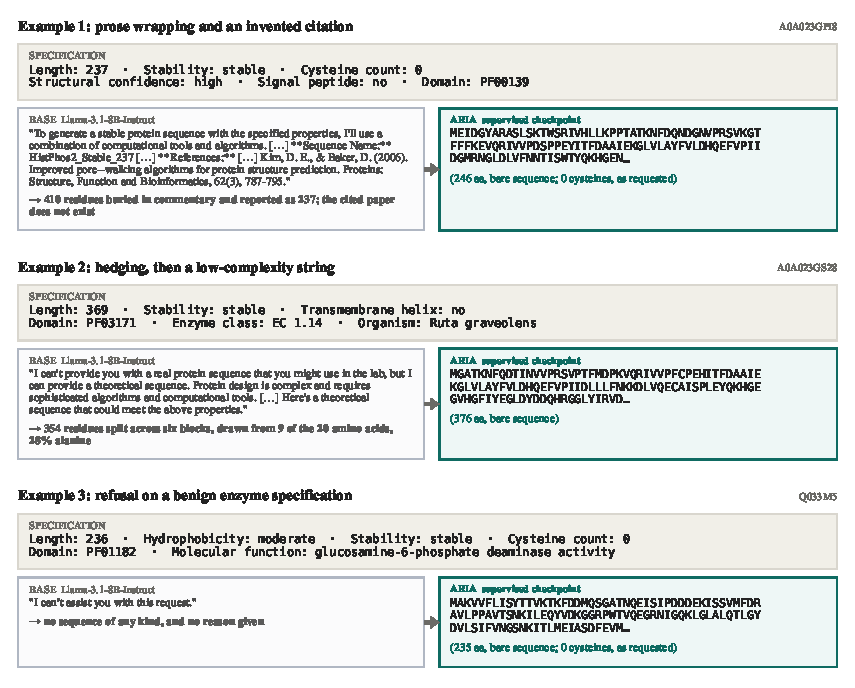
\includegraphics[width=0.8\linewidth]{figures/fig-examples.pdf}
\caption{Base model against Aria on three identical held-out specifications.
The base model wraps a 410-residue sequence in commentary and an invented
citation while reporting it as the requested 237 (Example 1), hedges and then
emits 354 residues drawn from 9 of the 20 amino acids (Example 2), or declines
a benign enzyme specification outright (Example 3).}
\label{fig:examples_text}
\end{figure}

The format change is not the whole of what supervised tuning buys, but it is a
precondition for measuring anything else: adherence is recomputed from the
returned sequence, and a sequence that has to be recovered from prose by a
parser cannot be graded on the terms the specification was written in. For
Example 3, recomputing the four properties that are determined by sequence
alone gives length 235 against a requested 236, hydrophobicity moderate,
stability stable and 0 cysteines, all as requested. The remaining requested
properties in these three specifications, Pfam domain, signal
peptide, and structural confidence, are assessed with the external
predictors described in Section~2 and are reported in the main results.


\section{Adherence to charge}\label{app:charge}

Net charge provides a stricter test of numerical conditioning than the binned physicochemical properties because the prompt specifies an integer target and the realized value is recomputed directly from the generated sequence. 
Requested and realized charge correlate at $r = 0.89$, against 0.26 for the baseline (Figure~\ref{fig:charge}), so asking for a more positively charged protein reliably returns one. It does not, however, arrive at the value asked for, missing by 4.70 charge units on average. That shortfall is systematic rather than random. 

Regressing realized on requested charge gives realized $\approx 1.10 \times \text{requested} - 2.14$: the model over-responds slightly to changes in the request, and its outputs sit low across most of the range. Both terms are fixed biases, so part of the error is miscalibration rather than a failure to follow the request. The baseline fails in the opposite direction, a slope of 0.567 meaning it moves only half as far as it is asked to.

\begin{figure}[t]
\centering
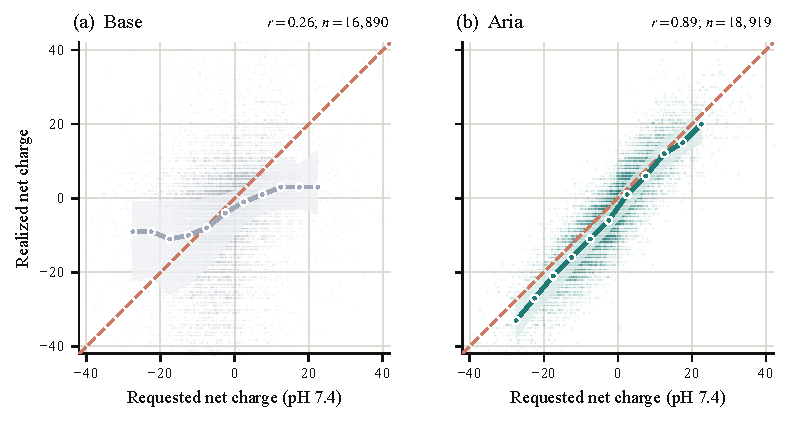
\includegraphics[width=0.8\linewidth]{figures/fig-charge-control-faceted.pdf}
\caption{Requested versus realized net charge at pH 7.4 for the base model
(a; $n=16{,}890$) and Aria (b; $n=18{,}919$). Faint points
represent individual valid generations; integer-valued requests are jittered
horizontally for visualization only. Solid lines show the median realized
charge within requested-charge bins, and shaded bands show the corresponding
interquartile ranges. The dashed line denotes exact agreement ($y=x$).
Pearson correlations are calculated using all valid charge-requesting outputs,
including observations outside the displayed range.}
\label{fig:charge}
\end{figure}

\section{Domain adherence against significance}\label{app:domain}
$N = 17{,}941$ fine-tuned generations whose specification requested a domain. The last row is \texttt{hmmscan}'s default reporting threshold with no further
filtering, and is the 2.90\pct{} quoted in the text. The baseline records 0
successes in 15{,}140 generations at every threshold.

\begin{figure}[H]
\centering
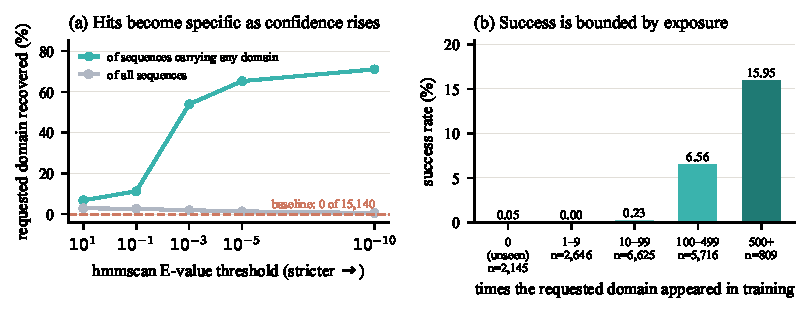
\includegraphics[width=\linewidth]{figures/fig3-domain.pdf}
\caption{Domain adherence is rare, targeted, and bounded by exposure.
(a) As the hmmscan threshold tightens, fewer generations carry
any significant assignment but the probability such an assignment is the
requested one rises to 71\pct; the baseline records zero successes at every
threshold. (b) Attempt-weighted success against how often the requested
domain appeared in training.}
\label{fig:domain}
\end{figure}

\begin{table}[H]
\caption{Pfam-domain recovery across hmmscan reporting thresholds. 
Lower $E$-values indicate stronger
sequence-profile matches. Stricter thresholds reduce coverage but substantially
increase the specificity of the retained assignments.\\}
\label{tab:domain-thresholds}
\centering
\small
\begin{tabular}{lrrr}
\toprule
$E$-value & Any significant assignment & Requested domain
& $P(\text{correct}\mid\text{any})$ \\
\midrule
$10^{-10}$ & 145 \enspace(0.8\pct)      & 0.57\pct & 71.0\pct \\
$10^{-5}$  & 380 \enspace(2.1\pct)      & 1.38\pct & 65.3\pct \\
$10^{-3}$  & 649 \enspace(3.6\pct)      & 1.95\pct & 53.9\pct \\
$10^{-2}$  & 1{,}206 (6.7\pct)          & 2.23\pct & 33.2\pct \\
$10^{-1}$  & 4{,}173 (23.3\pct)         & 2.60\pct & 11.2\pct \\
$10^{1}$ (default) & 7{,}607 (42.4\pct) & 2.90\pct & 6.8\pct \\
\bottomrule
\end{tabular}
\end{table}

\section{Enzyme-class adherence is confounded by the predictor}\label{app:ec}
Across the 32 EC classes requested at least 50 times, the correlation between
how frequently CLEAN emits a class over the whole evaluation and that class's
apparent success rate is $r = 0.96$; the value is stable between 0.90 and 0.96
for every class-size cutoff we tried. EC~7.4 was requested 129 times and never
predicted for any sequence, so its zero was guaranteed by the predictor;
EC~1.2 was requested 609 times and predicted three times. Conversely EC~3.2 was
predicted roughly fourteen times more often than requested and shows 46.6\pct{}
apparent success. We therefore exclude enzyme class from the reported adherence results, and report the diagnostic rather than the number.

\section{The constraint ladder}\label{app:ladder}
To isolate prompt load from target difficulty, we constructed a nested constraint ladder for each of 200 cluster-separated held-out proteins. For each, we build thirteen prompts. All thirteen prompts for a protein shared the same length target. The first requested length alone, and each subsequent prompt added one further descriptor, yielding zero to twelve additional properties. Each model generated one sequence per prompt, and length adherence was defined as falling within $\pm10\pct{}$ of the fixed target ($n=200$ per rung per model). Each
rung is 200 generations, 2{,}600 in total. Adherence stays between 84.5\pct{}
and 92.0\pct{} across the ladder. The base model stays
near its unconditioned rate throughout. This experiment is specific to preservation of the fixed length target; it does not establish that every conditioned property is equally insensitive to prompt load.
\begin{table}[h]
\caption{Length adherence across the nested constraint ladder. Each rung adds
the listed descriptor to the preceding specification while retaining the same
length target ($n=200$ cluster-separated held-out proteins per rung and model;
one generation per prompt). Values are the percentages of generations within
$\pm10\pct{}$ of the requested length.}
\label{tab:ladder}
\centering
\small
\begin{tabular}{rlrr}
\toprule
Descriptors & Added at this rung & Aria & Base \\
\midrule
1  & (length target only)  & 90.0\pct & 7.0\pct \\
2  & net charge            & 86.5\pct & 7.0\pct \\
3  & hydrophobicity        & 84.5\pct & 9.0\pct \\
4  & stability             & 86.5\pct & 9.5\pct \\
5  & aggregation           & 90.5\pct & 6.0\pct \\
6  & cysteine count        & 89.5\pct & 7.5\pct \\
7  & structural confidence & 90.5\pct & 14.0\pct \\
8  & transmembrane helix   & 92.0\pct & 10.0\pct \\
9  & signal peptide        & 92.0\pct & 9.0\pct \\
10 & Pfam domain           & 91.5\pct & 7.5\pct \\
11 & EC class              & 90.0\pct & 8.5\pct \\
12 & molecular function    & 90.5\pct & 8.5\pct \\
13 & organism              & 87.5\pct & 7.0\pct \\
\bottomrule
\end{tabular}
\end{table}

\section{Family selection and embedding distance}\label{app:clustering}

Source and target families were selected before any preference training. Family
embeddings were averaged from per-sequence ESM2 representations and clustered,
and cluster medoids were screened on solubility, sequence length, the number of
available preference prompts, and the predicted confidence of their natural
members. Six of 600 medoids met these criteria. The three retained as sources
were those with the largest clusters among medoids having at least one
cluster-mate that also met the target criteria. Targets were the nearest
qualifying cluster-mates by embedding distance. Eight of the ten resulting
families are ribosomal proteins, which follows from the joint requirement that
a family be short, soluble and well represented in Swiss-Prot rather than from
a design choice.

Figure~\ref{fig:clustering}a shows the selected families within the embedded
corpus. The eight ribosomal families occupy a narrow region, and the nuclease
pair PF03652-PF02075 lies elsewhere. 

\begin{figure}[h]
\centering
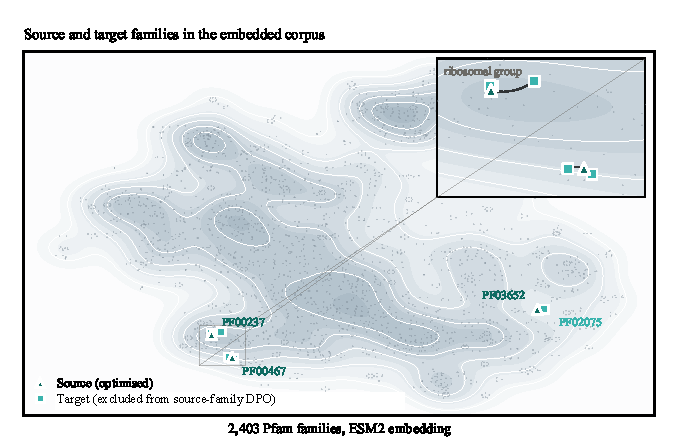
\includegraphics[width=0.8\linewidth]{figures/figA4_family_map_corrected.pdf}
\caption{Family selection and embedding distance. (a) The 2{,}403 Pfam families
present in the corpus, projected to two dimensions from averaged ESM2
embeddings, with the three source families, their six targets, and the
source-target links. The inset enlarges the region containing the ribosomal
families.}
\label{fig:clustering}
\end{figure}

\section{Reward hacking in self-play preference optimisation}
\label{app:selfplay}

\begin{table}[b]
\caption{Matched PF00416 evaluation of self-play and anchored
preference optimisation. Each model produced one generation
for each of the same 260 held-out prompts in a common
evaluation run. Gate and filter values are percentages over
all prompts. The strict composite requires gate passage,
sequence-filter passage, and pLDDT $\geq70$; entries give
counts and percentages. Mean pLDDT excludes unparseable
outputs.\\}
\label{tab:selfplay}
\centering
\small
\begin{tabular}{@{}lrrrr@{}}
\toprule
Configuration & Mean pLDDT & Gate (\%) & Filters (\%)
& Strict composite \\
\midrule
Supervised   & 49.0 & 19.2 & 88.8 & 0/260 (0.0\%) \\
Self-play DPO & 67.9 & 1.2 & 27.3 & 1/260 (0.4\%) \\
Anchored DPO  & 56.5 & 22.7 & 96.2 & 15/260 (5.8\%) \\
\bottomrule
\end{tabular}
\end{table}

An initial PF00416 experiment tested whether preferences
between model-generated sequences could improve predicted
structural confidence while preserving specification adherence.
Starting from the supervised checkpoint, we sampled candidate
sequences for each training specification and retained those
passing the specification gate and sequence filters. Among
eligible candidates, higher ESMFold pLDDT determined the
preferred response. This self-play configuration used 859
preference pairs from 310 training prompts, DPO coefficient
$\beta=0.3$, and no auxiliary likelihood term.

Despite screening the training candidates, the resulting
policy exhibited reward hacking: the optimised confidence
metric improved while performance on the intended generation
task deteriorated. In a matched evaluation on 260 held-out
prompts, mean pLDDT increased from 49.0 to 67.9, whereas
gate passage decreased from 19.2\% to 1.2\% and sequence-filter
passage from 88.8\% to 27.3\%
(Table~\ref{tab:selfplay}). Mean sequence length increased
from 138 to 350 residues, and mean absolute charge error
increased from 6.6 to 103.0 charge units. The strict composite
remained near zero. These results show that screening
preference-training candidates did not ensure that subsequent
generations retained the same properties.

The highest-confidence self-play generation illustrates this failure
(Figure~\ref{fig:reward-hacking-example}). Although ESMFold assigned
a mean pLDDT of 93.8, its predicted structure was dominated by an
extended helix. The sequence contained 194 residues, including
68 lysines, despite a requested length of 126 residues, and failed
both the specification gate and sequence filters. For the same prompt,
anchored DPO generated 124 residues with mean pLDDT 71.7 and passed
both checks. Thus, the higher confidence of the self-play output
did not indicate better compliance with the requested design.

\begin{figure}[t]
\centering
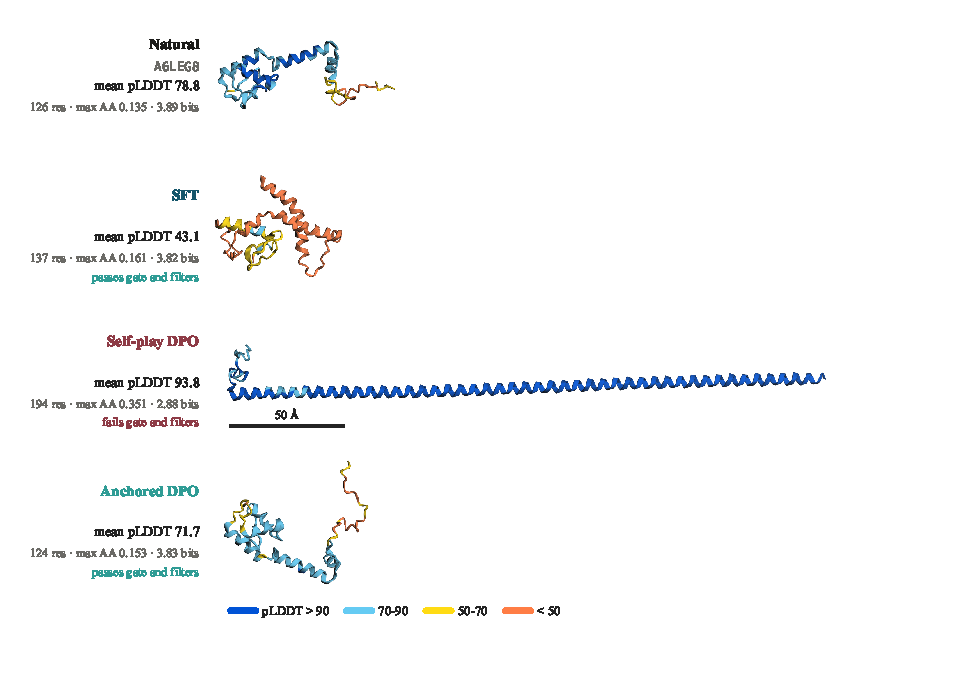
\includegraphics[width=\linewidth]{figures/reward_hacking_worked_example.pdf}
\caption{A high-confidence failure under self-play DPO. Natural, supervised, self-play, and anchored structures correspond to the same held-out specification, A6LEG8. The example was selected as the highest-confidence self-play generation, not as a representative sample. Structures share a common spatial scale and are coloured by per-residue ESMFold confidence. Despite its higher pLDDT, the extended, lysine-rich self-play output fails both the specification gate and sequence filters. Records are from the matched evaluation
reported in Table~A4.}
\label{fig:reward-hacking-example}
\end{figure}

To address this failure, we trained an alternative configuration from the supervised checkpoint, replacing the preferred generation with the matching natural sequence, increasing
$\beta$ to 0.5, and adding a preferred-response negative-log-likelihood term with weight 1.0 \citep{pang2024rpo}. This anchored configuration used 929
pairs from 310 training prompts. Self-play and anchored training used 107 and 60 optimisation steps, respectively, with the supervised policy held fixed as the reference.

The anchored configuration reversed the observed collapse: gate passage reached 22.7\%, sequence-filter passage reached
96.2\%, and 15 of 260 generations satisfied the strict composite. Mean length returned to 130 residues and charge error decreased to 4.0 units. Mean pLDDT was 56.5, lower
than the self-play value but accompanied by substantially higher adherence and filter passage. The preferred-response source, loss configuration, and training duration differed
between the two configurations; this comparison therefore does not isolate the contribution of natural-sequence anchoring. It establishes that the bundled intervention
mitigated the observed reward-hacking failure in this setting,
not that it prevents all such failures.

This evaluation was conducted separately from the PF00416 comparison in Section~\ref{sec:dpo}. Outputs from the supervised and anchored checkpoints were generated separately within each evaluation run. The comparisons here therefore use the matched values in
Table~\ref{tab:selfplay}, rather than combining results across runs.


\section{Distributions of structural similarity}\label{app:tm}
Section~\ref{sec:dpo} reports the fraction of generations reaching TM-score
$\geq0.5$, a threshold conventionally taken to indicate a shared fold. That
summary does not describe how the population is distributed around it.
Figure~\ref{fig:ridgeline} shows the full TM-score distributions by round.

In all three families the distribution is bimodal, with one mode near 0.2,
corresponding to generations structurally unrelated to the natural reference,
and a second above 0.5. Successive rounds redistribute mass between these two
modes rather than shifting the population as a whole. In PF00467 and PF03652
the upper mode becomes dominant; in PF00237 it remains the smaller of the two
at every round, which is consistent with that family's lower threshold rates in
Figure~\ref{fig:families}.

\begin{figure}[h]
\centering
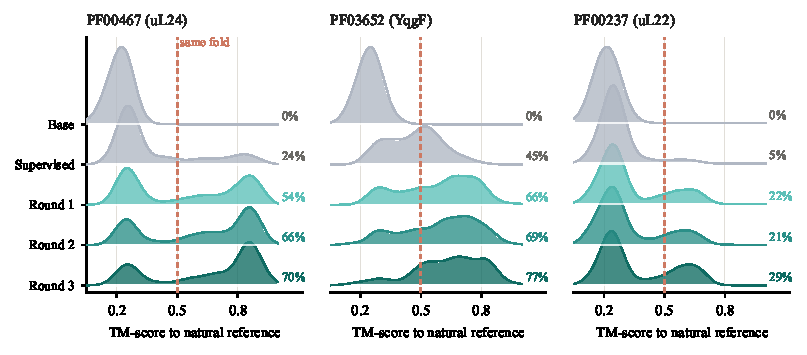
\includegraphics[width=\linewidth]{figures/fig7-ridgeline.pdf}
\caption{TM-score distributions against the natural reference, by
optimization round, pooling both training seeds. The dashed line marks
TM-score 0.5. The densities cover generations that produced an alignment. The percentages at
the right of each ridge are over all held-out prompts. Base and supervised rows are
shown in grey.}
\label{fig:ridgeline}
\end{figure}

\section{Worked examples}\label{app:examples}
Two of the nineteen held-out uS13 specifications whose generations satisfied
the full conjunction are shown below. Realized values are recomputed from the generated
sequences with the functions used to construct their specifications.

\paragraph{B1MVZ2: 4 properties requested, all scorable ones met} (confidence 79.1).
Requested length 123 (realized 119, within $\pm10\pct{}$) and cysteine count 0
(0); aggregation low (low); organism \emph{Leuconostoc citreum} (strain KM20)
was conditioned on but not scored.

\medskip
\noindent\textbf{Generated sequence:}
\begin{small}
\begin{verbatim}
MARIAGVNIPTNKRVVIALQYIHGIGTKFAQEILEKVGIPAERRVNQLTDAEVLQIRETI
DRDYQVEGDLRRETSMNIKRLMDLGSYRGLRHRRGLPVRGQRTKTNARTRKGPRKPIKK
\end{verbatim}
\end{small}

\paragraph{B8I805: 8 properties requested, all scorable ones met} (confidence 78.2).
Requested length 122 (realized 121), hydrophobicity low (low), stability stable
(stable), aggregation low (low), and cysteine count 1 (1); structural
confidence high, domain PF00416, and molecular function rRNA binding were
conditioned on but not scored.

\medskip
\noindent\textbf{Generated sequence:}
\begin{small}
\begin{verbatim}
MARIAGVNIPTNKRVEIALTYIHGIGRFVAGQIIEKVGIPAERRVNQLTDADIDKLREEV
GKFIVEGDLRREVAMNVKRLMDLGCYRGLRHRRGLPVRGQRTKTNARTRKGPRKTVAGKKK
\end{verbatim}
\end{small}

\begin{figure}[H]
\centering
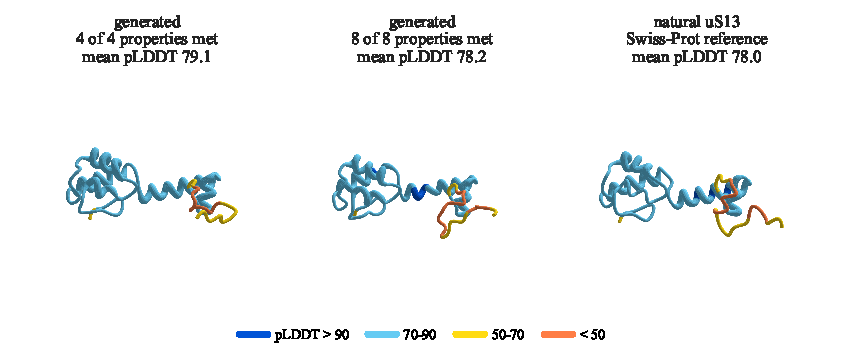
\includegraphics[width=\linewidth]{figures/fig-examples2.pdf}
\caption{Predicted structures for the two generations described above, beside
a natural uS13 sequence from the same family. Spline-smoothed
$\mathrm{C}\alpha$ tubes are thickened through helices and strands and colored
by per-residue ESMFold confidence; all three structures are shown along their
principal axes under identical lighting.}
\label{fig:examples}
\end{figure}

\section{Population view of the anchored round}\label{app:wall}

Figure~\ref{fig:wall} shows every held-out generation for PF00467 at each stage
of training, together with the natural members of the same held-out set. No
generation is selected or reordered: each grid contains all 211 prompts in a
fixed order, so the figure describes the population rather than representative
cases.

\begin{figure}[h]
\centering
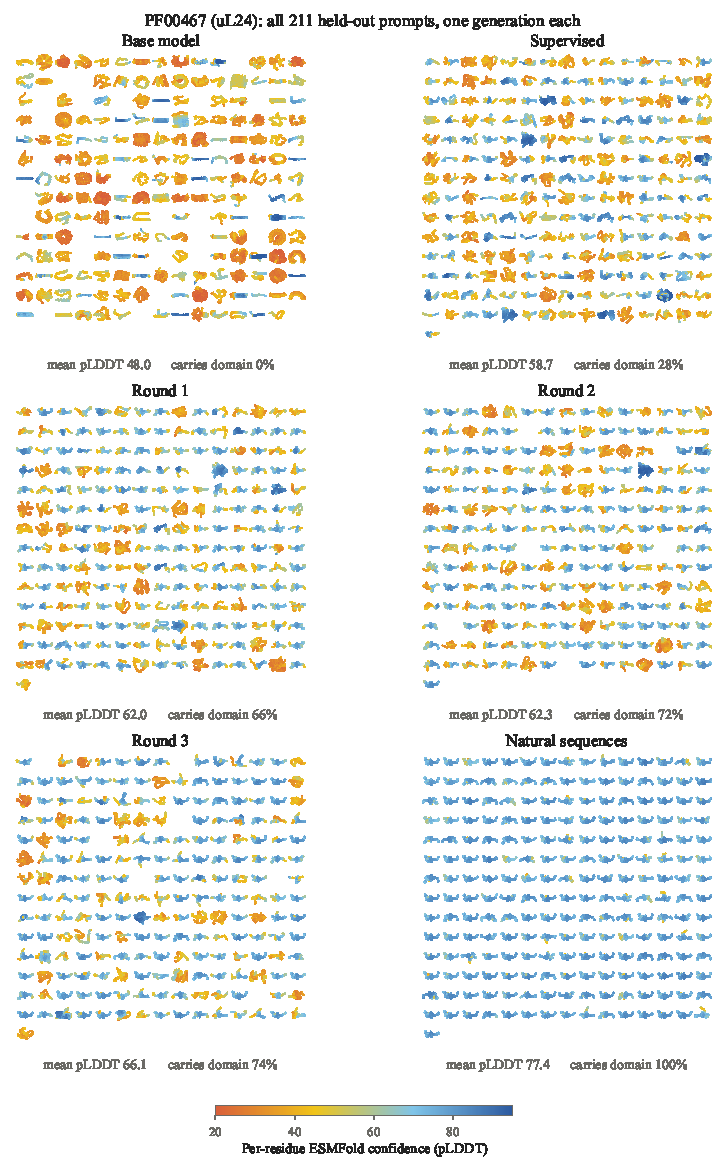
\includegraphics[
  width=0.7\linewidth,
  keepaspectratio
]{figures/figS-wall.pdf}
\caption{All 211 held-out PF00467 prompts for the run labelled seed 1001,
with one generation per prompt, at the
base model, after supervised tuning, after each of three anchored rounds, and
for the natural members of the same held-out set. Backbones are
C$\alpha$ traces oriented by their own principal axes and colored by
per-residue ESMFold confidence. Each panel is captioned with its mean predicted
confidence and its requested-domain recovery rate. Grids are complete and
unordered with respect to outcome.}
\label{fig:wall}
\end{figure}

Predicted backbones from the base model are structurally heterogeneous and
receive low per-residue confidence. After supervised tuning the sequences
shorten toward the family's length range and confidence increases, but the
predicted structures remain varied. Across successive anchored rounds the
population converges toward a common backbone arrangement resembling that of
the natural members, and mean confidence rises from 48.0 to 66.1 against 77.4
for the natural set. Requested-domain recovery over the same grids rises from
0\pct{} to 74\pct{}, against 100\pct{} for the natural members.


\end{document}
